% !TEX program = pdflatex
% !TeX encoding = utf8
% !TeX spellcheck = pl-PL

%%%%%%%%%%%%%%%%%%%%%%%%%%%%%%%%%%%%%%%%%%%%%%%%%%%%%%%%%%%%%%%%%%%%%%%%%%%
% Wybierz rodzaj pracy dyplomowej oraz wydział
% Pick thesis type and faculty
%%%%%%%%%%%%%%%%%%%%%%%%%%%%%%%%%%%%%%%%%%%%%%%%%%%%%%%%%%%%%%%%%%%%%%%%%%%
\documentclass[thesis=inz,faculty=ee]{EE-dyplom}

% thesis=[inz|mgr|bsc|msc]
%  * inz - praca inżynierska
%  * mgr - praca magisterska
%  * bsc - bachelor thesis
%  * msc - master thesis

% Skróty nazw wydziałów zgodne z domenami internetowymi
% Abbreviations of Faculties according to Internet subdomains
% faculty=[
%	arch,
%	gik,
%	ee,
%	wip
%	]

%%%%%%%%%%%%%%%%%%%%%%%%%%%%%%%%%%%%%%%%%%%%%%%%%%%%%%%%%%%%%%%%%%%%%%%%%%%
% Konfiguracja - do personalizacji
% Configuration - to be personalized
%%%%%%%%%%%%%%%%%%%%%%%%%%%%%%%%%%%%%%%%%%%%%%%%%%%%%%%%%%%%%%%%%%%%%%%%%%%
\instytut{Instytut Sterowania i Elektroniki Przemysłowej}
\kierunek{Informatyka Stosowana}
\specjalnosc{Inżynieria danych i multimedia}
\title{System do przetwarzania i archiwizacji strumieniowych danych finansowych w środowisku lokalnym}
\engtitle{A system for processing and archiving real-time financial data in an on-premises environment}
\album{325483}
\author{Maciej Karabin}
\promotor{mgr inż. Krzysztof Marek}
\date{2026}
\longdate{2026-01-01}

%%%%%%%%%%%%%%%%%%%%%%%%%%%%%%%%%%%%%%%%%%%%%%%%%%%%%%%%%%%%%%%%%%%%%%%%%%%
% Streszczenie pracy i abstract.
% In case of thesis in English swap the order - English version goes first.
%%%%%%%%%%%%%%%%%%%%%%%%%%%%%%%%%%%%%%%%%%%%%%%%%%%%%%%%%%%%%%%%%%%%%%%%%%%
\streszczeniepracy{
    Praca przedstawia projekt oraz implementację systemu do przetwarzania i archiwizacji strumieniowych danych
    finansowych z rynku kryptowalut w~środowisku lokalnym.
    Głównym celem jest zapewnienie wiarygodnego i kompletnego łańcucha przetwarzania danych, od odbioru, przez walidację
    i~wzbogacanie, aż po udostępnianie i archiwizację w trybie ciągłym.

    W ramach pracy zrealizowano architekturę opartą na mikrousługach, która integruje technologie takie jak Go, Docker,
    NATS JetStream, MongoDB oraz MinIO\@.
    System pobiera dane w czasie rzeczywistym z giełdy Binance za pomocą dedykowanego serwera strumieniowego.
    Następnie komunikaty są dystrybuowane przez brokera NATS JetStream do modułów ETL, które odpowiadają za ich
    transformację, oczyszczanie oraz wzbogacanie o metadane analityczne.
    Kluczowym elementem systemu jest mechanizm pamięci warstwowej (\textit{tiered storage}), który automatycznie
    przenosi dane historyczne z operacyjnej bazy danych MongoDB do archiwalnego magazynu obiektowego MinIO,
    optymalizując koszty i wydajność.
    Dostęp do surowych danych zapewnia interfejs GraphQL, a zintegrowany z platformą Telegram bot umożliwia
    wysyłanie powiadomień o zdarzeniach rynkowych.

    Struktura pracy obejmuje analizę istniejących rozwiązań i wymagań systemowych w rozdziale drugim.
    Rozdział trzeci szczegółowo opisuje zaprojektowaną architekturę systemu i przepływ danych między komponentami.
    Implementacja poszczególnych komponentów oraz wykorzystane technologie zostały przedstawione w rozdziale czwartym.
    Rozdział piąty wskazuje możliwe kierunki dalszego rozwoju systemu.
    Rozdział szósty dokumentuje przeprowadzone testy manualne weryfikujące poprawność działania systemu.
    Pracę kończy podsumowanie zawierające wnioski z realizacji projektu.
} % koniec streszczenia

\slowakluczowe{przetwarzanie strumieniowe, kryptowaluty, object storage, ETL, pamięć warstwowa, Go, NATS JetStream, EDA}

\thesisabstract{
    The thesis presents the design and implementation of a system for processing and archiving streaming financial data
    from the cryptocurrency market in an on-premises environment.
    The main objective is to ensure a reliable and complete data processing chain, from ingestion, through validation
    and enrichment, to continuous delivery and archiving.

    The project implements a microservices-based architecture that integrates technologies such as Go, Docker, NATS
    JetStream, MongoDB, and MinIO\@.
    The system fetches real-time data from the Binance exchange using a dedicated streaming server.
    Subsequently, the NATS JetStream broker distributes messages to ETL modules, which are responsible for their
    transformation, cleansing, and enrichment with analytical metadata.
    A key element of the system is the tiered storage mechanism, which automatically moves historical data from the
    operational MongoDB database to the archival MinIO object storage, optimizing costs and performance.
    Access to raw data is provided by a GraphQL interface, and a Telegram bot integrated with the platform enables
    sending notifications about market events.

    The structure of the thesis includes an analysis of existing solutions and system requirements in the second chapter.
    The third chapter describes the designed system architecture and data flow between components in detail.
    The implementation of individual components and the technologies used are presented in the fourth chapter.
    The fifth chapter indicates possible directions for further development of the system.
    The sixth chapter documents the manual tests conducted to verify the correct operation of the system.
    The thesis concludes with a summary that includes conclusions from the project.
} % end of abstract

\thesiskeywords{stream processing, cryptocurrency, object storage, ETL, tiered storage, Go, NATS JetStream, Event Driven Architecture}

%%%%%%%%%%%%%%%%%%%%%%%%%%%%%%%%%%%%%%%%%%%%%%%%%%%%%%%%%%%%%%%%%%%%%%%%%%%
% Pakiet float - umożliwia użycie [H] do wymuszenia pozycji obrazków
%%%%%%%%%%%%%%%%%%%%%%%%%%%%%%%%%%%%%%%%%%%%%%%%%%%%%%%%%%%%%%%%%%%%%%%%%%%
\usepackage{float}

%%%%%%%%%%%%%%%%%%%%%%%%%%%%%%%%%%%%%%%%%%%%%%%%%%%%%%%%%%%%%%%%%%%%%%%%%%%
% Tu zaczyna się dokument
% Here is the beginning of the document
%%%%%%%%%%%%%%%%%%%%%%%%%%%%%%%%%%%%%%%%%%%%%%%%%%%%%%%%%%%%%%%%%%%%%%%%%%%
\begin{document}
    % Strony nagłówkowe - musi być
    % Headers - must exist
    \frontpages

    % Tekst pracy - osobne pliki do edycji
    % Thesis text - separate files for edition
    \setcounter{page}{1}

    \chapter{Wstęp}

\label{ch:wstep}


\section{Wprowadzenie}

Dynamiczny rozwój rynku kryptowalut oraz jego wysoka zmienność powodują, że~organizacje finansowe potrzebują wiarygodnych strumieni danych o~niskim opóźnieniu.
Rynek ten generuje dzienny wolumen transakcyjny rzędu dziesiątek miliardów dolarów~\cite{coingecko}.
Jednocześnie specyfika giełd cyfrowych niesie ze~sobą ryzyka związane z~jakością danych.
Zjawiska takie jak \textit{wash trading}, czyli sztuczne generowanie obrotu, mogą prowadzić do~zafałszowania informacji rynkowych, przez co~publicznie dostępne, niesprawdzone dane mogą okazać się niewiarygodne~\cite{wash_trading}.
W~konsekwencji podmioty analizujące rynek, w~szczególności w~kontekście wykrywania anomalii czy~okazji arbitrażowych, nie~mogą opierać się wyłącznie na~zewnętrznych agregatorach, lecz powinny budować własne potoki przetwarzania danych (\textit{data pipelines})~\cite{arbitrage_finance}.

Ciągły dostęp do~danych historycznych i~strumieniowych jest fundamentem algorytmicznych strategii inwestycyjnych.
W~środowiskach o~ograniczonym zaufaniu do~sieci zewnętrznej istotna staje się także możliwość autonomicznego działania systemu (\textit{disconnected operations}), co~wpisuje się w~założenia przetwarzania brzegowego (\textit{edge computing})~\cite{edge_computing_satya}.

Projektowana architektura obejmuje serwer strumieniowy nasłuchujący kanałów WebSocket giełdy Binance, usługę wymiany komunikatów JetStream, moduły \textit{ETL} odpowiedzialne za~transformację i~wzbogacanie danych oraz warstwę analityczną udostępniającą zagregowane metryki.
Dostęp do~danych zapewnia interfejs GraphQL, natomiast bot platformy Telegram odpowiada za~dystrybucję powiadomień o~zdarzeniach rynkowych w~czasie rzeczywistym.

Kluczowym elementem infrastruktury jest mechanizm \textit{tiered storage} (pamięć warstwowa).
Dane w~systemie trafiają najpierw do~warstwy gorącej (MongoDB), a~następnie~-- po~upływie określonego czasu retencji~-- przenoszone są do~warstwy zimnej opartej na~MinIO. Pozwala to~odciążyć bazę operacyjną, obniżyć koszty przechowywania danych historycznych oraz zwiększyć niezawodność przetwarzania~\cite{unity_tiered_storage}.
W~warstwie obiektowej dane mogą być dodatkowo kompresowane i~wersjonowane.


\section{Cel pracy}

Celem pracy jest zaprojektowanie i~implementacja kompletnego łańcucha przetwarzania danych rynkowych obejmującego odbiór, walidację, wzbogacanie, udostępnianie oraz archiwizację informacji w~trybie ciągłym.
W~ramach pracy został opracowany niezawodny serwer strumieniowy utrzymujący połączenia z~WebSocket Binance.
Zaprojektowano kanał dystrybucyjny oparty na~NATS JetStream, zapewniający buforowanie zdarzeń oraz odporność na~awarie usług zależnych.
Zaimplementowano procesy \textit{ETL} dzielące dane na~zbiory surowe i~oczyszczone oraz wzbogacające je~o~metadane analityczne.
Skonfigurowano i~zautomatyzowano przenoszenie danych w~modelu \textit{tiered storage} (MongoDB~→~MinIO), zapewniając optymalizację zasobów warstwy operacyjnej przy równoczesnej dostępności danych historycznych.
Zintegrowano system powiadomień z~Telegramem, umożliwiając przesyłanie alertów rynkowych w~czasie rzeczywistym.

Realizacja założeń obejmuje przygotowanie dokumentacji architektury, implementację usług w~języku \textit{Go} oraz konfigurację infrastruktury w~środowisku Docker.


\section{Plan pracy}

Niniejsza praca składa się z~siedmiu rozdziałów, z~czego pierwszy stanowi wprowadzenie do~problematyki, kolejne cztery opisują realizację systemu, zaś dwa ostatnie podsumowują osiągnięte rezultaty oraz wskazują kierunki dalszego rozwoju.

W~rozdziale~\ref{ch:analiza} przedstawiono analizę wymagań funkcjonalnych i~niefunkcjonalnych systemu, obejmującą m.in.\ minimalne opóźnienia przetwarzania, odporność na~awarie oraz skalowalność infrastruktury.
Dokonano przeglądu istniejących rozwiązań w~obszarze przetwarzania danych finansowych, w~tym platform strumieniowych takich jak Apache Kafka czy~NATS JetStream, oraz porównano mechanizmy składowania danych w~architekturach warstwowych.
Rozdział zawiera także uzasadnienie wyboru technologii wykorzystanych w~projekcie.

Rozdział~\ref{ch:projekt} zawiera szczegółowy projekt architektury systemu, obejmujący dekompozycję na~warstwy: pozyskiwania danych, przetwarzania strumieniowego, transformacji \textit{ETL}, składowania oraz udostępniania.
Opisano strukturę baz danych MongoDB przechowujących dane operacyjne oraz~konfigurację warstwy obiektowej MinIO jako pamięci zimnej.
Przedstawiono przepływ danych między poszczególnymi komponentami, mechanizmy komunikacji asynchronicznej przez kolejki \textit{JetStream} oraz zasady wersjonowania i~retencji danych.
Rozdział uwzględnia także schemat połączenia z~interfejsem GraphQL oraz integracją z~API Telegrama w~celu dystrybucji powiadomień.

Rozdział~\ref{ch:implementacja} przedstawia szczegóły implementacyjne systemu, w~tym wybrane biblioteki języka \textit{Go} do~obsługi WebSocket, deserializacji JSON oraz interakcji z~bazami danych.
Opisano napotkane problemy, takie jak zarządzanie ponownymi połączeniami po~awariach, obsługa backpressure w~strumieniach danych czy~optymalizacja zapytań do~MongoDB przy dużym wolumenie rekordów.
Zaprezentowano także fragmenty kodu źródłowego ilustrujące kluczowe mechanizmy, w~szczególności logikę archiwizacji danych oraz~konstrukcję (\textit{resolverów}) GraphQL\@.

Rozdział~\ref{sec:rozwoj} wskazuje możliwe kierunki dalszego rozwoju systemu, obejmujące rozszerzenie o~dodatkowe giełdy kryptowalut, zastosowanie algorytmów wykrywania anomalii oraz integrację z~systemami monitoringu i~powiadamiania, takimi jak Prometheus czy~Grafana.
Rozważono także możliwość wdrożenia mechanizmów uczenia maszynowego do~predykcji ruchów cenowych oraz automatycznego generowania zleceń handlowych na~podstawie analizy danych historycznych.

Rozdział~\ref{ch:testy} dokumentuje przeprowadzone testy manualne weryfikujące poprawność działania poszczególnych komponentów.
Opisano scenariusze testowe obejmujące m.in.\ odbiór danych z~WebSocket, transformację rekordów w~procesach \textit{ETL}, obsługę awarii komponentów oraz poprawność odpowiedzi GraphQL\@.
Przedstawiono wyniki pomiarów opóźnień w~łańcuchu przetwarzania oraz statystyki dotyczące wolumenu przetwarzanych danych.

Pracę zamyka rozdział~\ref{ch:podsumowanie}, w~którym podsumowano rezultaty projektu, omówiono stopień realizacji założonych celów oraz~wskazano wnioski płynące z~realizacji systemu.
Zidentyfikowano mocne strony zaprojektowanej architektury, takie jak modularność, odporność na~awarie oraz niskie koszty operacyjne, a~także obszary wymagające dalszych udoskonaleń.


    \chapter{Przetwarzanie danych strumieniowych}
\label{ch:przetwarzanie_danych}

Niniejszy rozdział przedstawia teoretyczne podstawy przetwarzania danych strumieniowych, ze~szczególnym uwzględnieniem
specyfiki rynków finansowych i~kryptowalutowych.
Omówiono kluczowe koncepcje, modele przetwarzania oraz wyzwania związane z~obsługą ciągłych przepływów danych
w~czasie rzeczywistym.


\section{Charakterystyka danych strumieniowych}
\label{sec:charakterystyka_strumieni}

Dane strumieniowe (\textit{streaming data}) to~ciągły, potencjalnie nieskończony przepływ rekordów generowanych
w~czasie rzeczywistym przez różnorodne źródła.
W~odróżnieniu od~tradycyjnych zbiorów danych o~skończonym rozmiarze, strumienie charakteryzują się brakiem określonego
początku i~końca --- nowe dane napływają nieprzerwanie, a~ich przetwarzanie musi odbywać się na~bieżąco~\cite{data_stream_def}.

W~kontekście rynków kryptowalutowych dane strumieniowe obejmują przede wszystkim zdarzenia transakcyjne
(\textit{trade events}), aktualizacje arkuszy zleceń (\textit{order book updates}) oraz zmiany cen i~wolumenów.
Giełdy takie jak Binance generują tysiące komunikatów na~sekundę dla~popularnych par handlowych, co~stawia wysokie
wymagania przed systemami przetwarzającymi.

Kluczowe cechy danych strumieniowych z~rynków finansowych to~\cite{burst_events, time_value_curve, 8_requirements}:
\begin{itemize}
    \item \textbf{Wysoka częstotliwość} --- komunikaty napływają w~odstępach milisekundowych, szczególnie w~okresach
    zwiększonej zmienności rynkowej.
    \item \textbf{Zmienność natężenia} --- przepływ danych nie~jest stały; w~momentach publikacji istotnych informacji
    rynkowych wolumen komunikatów może wzrosnąć wielokrotnie.
    \item \textbf{Krytyczność czasowa} --- wartość informacji maleje wraz z~upływem czasu; opóźnione dane tracą
    użyteczność dla~algorytmów handlowych.
\end{itemize}


\section{Modele przetwarzania danych}
\label{sec:modele_przetwarzania}

W~literaturze i~praktyce inżynierskiej wyróżnia się dwa podstawowe podejścia do~przetwarzania danych: przetwarzanie
wsadowe (\textit{batch processing}) oraz przetwarzanie strumieniowe (\textit{stream processing}).
Każde z~nich charakteryzuje się odmiennymi właściwościami i~znajduje zastosowanie w~różnych scenariuszach.

\subsection{Przetwarzanie wsadowe}
\label{subsec:batch_processing}

Przetwarzanie wsadowe polega na~gromadzeniu danych przez~określony czas, a~następnie ich jednorazowym przetworzeniu
jako~skończonego zbioru.
Model ten jest dobrze ugruntowany i~szeroko stosowany w~systemach analitycznych, gdzie~akceptowalne są~opóźnienia
rzędu minut, godzin lub~dni.

Typowy przepływ przetwarzania wsadowego obejmuje ekstrakcję danych ze~źródeł, ich~transformację zgodnie z~logiką
biznesową oraz~załadowanie do~docelowego magazynu danych (\textit{ETL --- Extract, Transform, Load}).
Procesy te~uruchamiane są~cyklicznie, według ustalonego harmonogramu.

Zalety przetwarzania wsadowego to~prostota implementacji, łatwość debugowania oraz~możliwość ponownego przetworzenia
całego zbioru w~przypadku wykrycia błędów.
Wadą jest natomiast opóźnienie między~powstaniem danych a~ich dostępnością dla~odbiorców, co~w~kontekście rynków
finansowych może być nieakceptowalne~\cite{bigdata_principles}.

\subsection{Przetwarzanie strumieniowe}
\label{subsec:stream_processing}

Przetwarzanie strumieniowe zakłada przetwarzanie danych natychmiast po~ich nadejściu, bez~oczekiwania na~zgromadzenie
pełnego zbioru.
Każdy komunikat jest analizowany indywidualnie lub~w~kontekście niewielkiego okna czasowego, a~wyniki są~udostępniane
z~minimalnym opóźnieniem.

W~tym modelu dane przepływają przez~zdefiniowany potok przetwarzania (\textit{pipeline}), składający się z~operatorów
realizujących transformacje, filtrowanie, agregację czy~wzbogacanie rekordów.
Strumień wyjściowy może być kierowany do~kolejnych etapów przetwarzania, zapisywany w~bazie danych lub~wykorzystywany
do~generowania alertów.

Przetwarzanie strumieniowe jest szczególnie istotne w~kontekście danych finansowych, gdzie~opóźnienia rzędu
milisekund mogą decydować o~rentowności strategii handlowych.
Wymaga jednak bardziej złożonej infrastruktury oraz~starannego zarządzania stanem przetwarzania~\cite{8_requirements}.

\subsection[Architektura Lambda i Kappa]{Architektura Lambda i~Kappa}
\label{subsec:lambda_kappa}

W~praktyce często stosuje się architektury hybrydowe, łączące zalety obu podejść.
Architektura Lambda zakłada równoległe działanie dwóch ścieżek przetwarzania: warstwy wsadowej (\textit{batch layer})
zapewniającej kompletność i~poprawność danych historycznych oraz~warstwy strumieniowej (\textit{speed layer})
dostarczającej wyniki w~czasie rzeczywistym.
Warstwa udostępniania (\textit{serving layer}) łączy wyniki z~obu ścieżek, udostępniając spójny widok danych~\cite{bigdata_principles}.

Architektura Kappa stanowi uproszczenie tego modelu poprzez eliminację dedykowanej warstwy wsadowej.
W~tym podejściu wszystkie dane są~przetwarzane jako~strumień, a~przetwarzanie historyczne realizowane jest poprzez
ponowne odtworzenie strumienia z~trwałego magazynu zdarzeń.
Model ten jest koncepcyjnie prostszy, lecz~wymaga odpowiedniej infrastruktury do~przechowywania i~odtwarzania
historycznych strumieni~\cite{kappa_architecture}.


\section{Semantyka dostarczania komunikatów}
\label{sec:semantyka_dostarczania}

Kluczowym aspektem systemów przetwarzania strumieniowego jest semantyka dostarczania komunikatów, określająca
gwarancje dotyczące tego, ile~razy każdy komunikat zostanie przetworzony.
Wyróżnia się trzy podstawowe poziomy gwarancji:

\subsection[At-most-once (co najwyżej raz)]{At-most-once (co~najwyżej raz)}
\label{subsec:at_most_once}

W~semantyce \textit{at-most-once} komunikat może zostać utracony, lecz~nigdy nie~zostanie przetworzony więcej
niż~jeden raz.
Jest to~najprostsza do~implementacji gwarancja, gdyż~nie wymaga mechanizmów potwierdzeń ani~powtórzeń.
Stosowana jest w~scenariuszach, gdzie~sporadyczna utrata danych jest~akceptowalna, na~przykład w~systemach
monitoringu, gdzie~pojedyncze brakujące pomiary nie~wpływają istotnie na~ogólny obraz.

W~kontekście danych finansowych semantyka ta~jest rzadko stosowana, ponieważ utrata nawet pojedynczej transakcji
może prowadzić do~niespójności w~analizach lub~błędnych decyzji inwestycyjnych~\cite{at_least_once}.

\subsection[At-least-once (co najmniej raz)]{At-least-once (co~najmniej raz)}
\label{subsec:at_least_once}

Semantyka \textit{at-least-once} gwarantuje, że~każdy komunikat zostanie przetworzony przynajmniej jeden raz,
lecz~dopuszcza możliwość duplikatów.
Realizowana jest poprzez mechanizm potwierdzeń (\textit{acknowledgements}) --- komunikat pozostaje w~kolejce do~czasu
otrzymania potwierdzenia pomyślnego przetworzenia.
W~przypadku awarii konsumenta lub~braku potwierdzenia, komunikat jest dostarczany ponownie.

Model ten wymaga, aby~konsumenci byli idempotentni, czyli~wielokrotne przetworzenie tego samego komunikatu
nie~powinno prowadzić do~niepożądanych efektów ubocznych.
W~praktyce idempotentność osiąga się poprzez deduplikację na~podstawie unikalnych identyfikatorów komunikatów
lub~projektowanie operacji w~sposób naturalnie idempotentny (np.~ustawianie wartości zamiast inkrementacji)~\cite{at_least_once}.

\subsection{Exactly-once (dokładnie raz)}
\label{subsec:exactly_once}

Semantyka \textit{exactly-once} stanowi najsilniejszą gwarancję --- każdy komunikat jest przetwarzany dokładnie
jeden raz, bez~utraty i~bez~duplikatów.
Jest to~najbardziej pożądana, lecz~zarazem najtrudniejsza do~osiągnięcia semantyka.

Realizacja wymaga koordynacji między~producentem, brokerem i~konsumentem, często z~wykorzystaniem mechanizmów
transakcyjnych lub~rozproszonego zatwierdzania (\textit{distributed commit}).
Ze~względu na~złożoność implementacji oraz~wpływ na~wydajność, w~wielu systemach stosuje się semantykę
\textit{at-least-once} w~połączeniu z~idempotentnym przetwarzaniem jako~praktyczny kompromis~\cite{at_least_once}.


\section[Okna czasowe w przetwarzaniu strumieniowym]{Okna czasowe w~przetwarzaniu strumieniowym}
\label{sec:okna_czasowe}

Wiele operacji analitycznych wymaga agregacji danych w~określonych przedziałach czasowych.
W~przetwarzaniu strumieniowym wykorzystuje się koncepcję okien czasowych, które~grupują zdarzenia na~potrzeby obliczeń zbiorczych.

\subsection{Okna stałe (fixed windows)}
\label{subsec:fixed_windows}

Okna stałe dzielą strumień na~rozłączne, następujące po~sobie przedziały o~jednakowej długości.
Każde zdarzenie należy do~dokładnie jednego okna, a~wyniki agregacji są~emitowane po~zamknięciu każdego okna.

Przykładem zastosowania jest obliczanie średniej ceny w~interwałach minutowych --- każda minuta stanowi osobne okno,
a~po jej~zakończeniu publikowany jest wynik (np.~cena otwarcia, zamknięcia, maksimum, minimum).
Takie agregaty stanowią podstawę wykresów świecowych (\textit{candlestick charts}) powszechnie stosowanych
w~analizie technicznej~\cite{dataflow_model}.

\subsection{Okna przesuwne (sliding windows)}
\label{subsec:sliding_windows}

Okna przesuwne obejmują zdarzenia z~określonego przedziału czasowego, lecz~w~odróżnieniu od~okien stałych,
nakładają się na~siebie.
Okno przesuwa się wraz z~nadejściem nowych zdarzeń, umożliwiając ciągłą aktualizację wyników agregacji.

Typowym zastosowaniem jest obliczanie średniej kroczącej (\textit{moving average}), gdzie~wynik jest aktualizowany
przy~każdym nowym zdarzeniu, uwzględniając ostatnie N~minut lub~ostatnie N~transakcji.
Okna przesuwne zapewniają płynniejszy obraz zmian, lecz~wymagają większych zasobów obliczeniowych ze~względu
na~nakładanie się przedziałów~\cite{dataflow_model}.

\subsection{Okna sesyjne (session windows)}
\label{subsec:session_windows}

Okna sesyjne grupują zdarzenia na~podstawie aktywności, a~nie sztywnych granic czasowych.
Sesja rozpoczyna się wraz z~pierwszym zdarzeniem i~trwa do~momentu, gdy~przez~zdefiniowany okres nie~napłyną żadne
nowe zdarzenia (tzw.~\textit{gap}).
Po~przekroczeniu tego progu sesja jest zamykana, a~kolejne zdarzenie rozpoczyna nową sesję.

W~kontekście rynków finansowych okna sesyjne mogą być wykorzystywane do~identyfikacji okresów wzmożonej aktywności
handlowej lub~grupowania serii szybkich transakcji wykonywanych przez~algorytmy wysokiej częstotliwości~\cite{dataflow_model}.


\section[Problemy i wyzwania]{Problemy i~wyzwania}
\label{sec:problemy_strumieniowe}

Przetwarzanie danych strumieniowych wiąże się z~szeregiem wyzwań technicznych i~koncepcyjnych, które~wymagają
starannego rozwiązania na~etapie projektowania systemu.

\subsection{Zarządzanie czasem zdarzeń}
\label{subsec:czas_zdarzen}

W~systemach rozproszonych rozróżnia się czas zdarzenia (\textit{event time}), czyli~moment faktycznego wystąpienia
zdarzenia u~źródła, oraz~czas przetwarzania (\textit{processing time}), czyli~moment dotarcia zdarzenia do~systemu.
Różnica między~tymi znacznikami wynika z~opóźnień sieciowych, kolejkowania oraz~ewentualnych awarii.

Zdarzenia mogą docierać w~kolejności innej niż~chronologiczna (tzw.~\textit{out-of-order events}), co~komplikuje
obliczenia oparte na~czasie.
System musi decydować, jak~długo czekać na~potencjalnie opóźnione zdarzenia przed zamknięciem okna czasowego
i~emisją wyników.
Zbyt~krótkie oczekiwanie prowadzi do~pominięcia opóźnionych danych, zbyt~długie --- do~zwiększenia opóźnienia wyników.

Mechanizm \textit{watermarks} pozwala śledzić postęp czasu zdarzeń i~sygnalizować, że~wszystkie zdarzenia
o~znaczniku czasowym mniejszym od~pewnej wartości zostały już~odebrane.
Zdarzenia przychodzące po~przekroczeniu znacznika czasu są~traktowane jako~spóźnione i~mogą być odrzucane
lub~przetwarzane w~specjalny sposób~\cite{dataflow_model}.

\subsection{Zarządzanie stanem}
\label{subsec:zarzadzanie_stanem}

Wiele operacji strumieniowych wymaga utrzymywania stanu między~kolejnymi komunikatami --- na~przykład obliczenie
średniej kroczącej wymaga pamiętania poprzednich wartości, a~agregacja w~oknie czasowym --- gromadzenia zdarzeń
do~momentu zamknięcia okna.

Zarządzanie stanem w~systemach rozproszonych jest wyzwaniem ze~względu na~konieczność zapewnienia trwałości
(stan nie~może zostać utracony w~przypadku awarii), spójności (wszystkie repliki muszą widzieć ten~sam stan)
oraz~wydajności (dostęp do~stanu nie~może stanowić wąskiego gardła).

Stosowane podejścia obejmują lokalne magazyny stanu z~mechanizmem punktów kontrolnych (\textit{checkpointing}),
zewnętrzne bazy danych o~niskich opóźnieniach oraz~rozproszone struktury danych z~replikacją~\cite{flink}.

\subsection[Backpressure i kontrola przepływu]{Backpressure i~kontrola przepływu}
\label{subsec:backpressure}

Sytuacja, w~której producent generuje dane szybciej niż~konsument jest w~stanie je~przetworzyć, nazywana jest
przeciążeniem (\textit{backpressure}).
Bez~odpowiednich mechanizmów kontroli przepływu system może ulec destabilizacji --- kolejki rosną nieograniczenie,
pamięć się wyczerpuje, a~opóźnienia stale się~zwiększają.

Strategie radzenia sobie z~backpressure obejmują buforowanie z~ograniczeniem rozmiaru (nadmiarowe komunikaty
są~odrzucane), adaptacyjne spowalnianie producenta (poprzez sygnalizację zwrotną), oraz~skalowanie horyzontalne
konsumentów (dodawanie kolejnych instancji przetwarzających)~\cite{google_sre_book}.

W~kontekście danych z~rynków kryptowalutowych backpressure może wystąpić w~okresach ekstremalnej zmienności,
gdy~wolumen transakcji wielokrotnie przekracza typowe wartości.
System musi być~zaprojektowany tak, aby~degradował wydajność (zwiększając opóźnienie) zamiast tracić dane lub~ulegać
całkowitej awarii.

\subsection[Skalowalność i partycjonowanie]{Skalowalność i~partycjonowanie}
\label{subsec:skalowalnosc}

Skalowanie systemów strumieniowych wymaga możliwości podziału strumienia na~niezależne partycje, które~mogą być
przetwarzane równolegle.
Kluczem partycjonowania jest zazwyczaj atrybut danych zapewniający równomierny rozkład obciążenia oraz~zachowanie
lokalności danych powiązanych logicznie~\cite{scaling}.

W~przypadku danych z~giełd kryptowalut naturalnym kluczem partycjonowania jest symbol pary handlowej --- wszystkie
zdarzenia dotyczące danej pary (np.~BTCUSDT) trafiają do~tej~samej partycji, co~umożliwia lokalne obliczanie
agregatów bez~koordynacji między~partycjami.

Wyzwaniem jest zapewnienie równomiernego rozkładu obciążenia, gdy~popularność poszczególnych par jest zróżnicowana.
Para BTC/USDT generuje znacznie więcej transakcji niż~mniej popularne pary, co~może prowadzić do~nierównomiernego
obciążenia partycji (\textit{hot spots})~\cite{coingecko}.


\section{Architektura sterowana zdarzeniami}
\label{sec:event_driven}

Architektura sterowana zdarzeniami (\textit{Event-Driven Architecture}, EDA) stanowi paradygmat projektowania
systemów, w~którym przepływ sterowania jest determinowany przez~zdarzenia --- sygnały o~wystąpieniu określonych
stanów lub~akcji w~systemie.

W~modelu tym komponenty systemu komunikują się poprzez publikowanie i~subskrybowanie zdarzeń, bez~bezpośrednich
wywołań synchronicznych.
Producent zdarzenia nie~musi znać odbiorców, a~konsumenci mogą dołączać lub~odłączać się dynamicznie,
co~zapewnia luźne powiązanie (\textit{loose coupling}) między~modułami~\cite{edd_pub_sub}.

Centralna rola w~architekturze EDA przypada brokerowi wiadomości, który~odpowiada za~przyjmowanie zdarzeń
od~producentów, ich~trwałe przechowywanie oraz~dostarczanie do~zainteresowanych konsumentów.
Broker zapewnia buforowanie w~przypadku chwilowej niedostępności odbiorców oraz~może realizować dodatkowe
funkcje, takie jak~filtrowanie, routing czy~transformacja komunikatów~\cite{data_broker}.

Zalety architektury sterowanej zdarzeniami obejmują naturalną asynchroniczność (operacje nie~blokują się wzajemnie),
łatwość dodawania nowych konsumentów (bez~modyfikacji istniejących komponentów), oraz~odporność na~awarie
(zdarzenia są~buforowane do~czasu pomyślnego przetworzenia).
Głównymi wadami są~większa złożoność debugowania (brak liniowego przepływu sterowania) oraz~konieczność zarządzania
ostateczną spójnością (\textit{eventual consistency})~\cite{fundamentals}.


\section{Podsumowanie}
\label{sec:podsumowanie_przetwarzanie}

Przetwarzanie danych strumieniowych z~rynków finansowych wymaga starannego doboru modeli, semantyk i~mechanizmów
odpowiadających specyfice tego~obszaru.
Kluczowe znaczenie ma~minimalizacja opóźnień, zapewnienie niezawodności dostarczania oraz~elastyczna obsługa
zmiennego obciążenia.

Architektura sterowana zdarzeniami w~połączeniu z~semantyką dostarczania \textit{at-least-once} i~idempotentnym
przetwarzaniem stanowi praktyczny kompromis między~złożonością implementacji a~wymaganymi gwarancjami.
Mechanizmy okien czasowych umożliwiają realizację analiz agregacyjnych, natomiast odpowiednie strategie
partycjonowania i~kontroli przepływu zapewniają skalowalność systemu.

W~kolejnych rozdziałach przedstawiono, w~jaki sposób opisane koncepcje zostały zastosowane w~projektowanym systemie
do~przetwarzania danych z~giełdy kryptowalut Binance.


    \chapter{Analiza wymagań}
\label{ch:analiza}

Niniejszy rozdział przedstawia analizę wymagań oraz projekt systemu do przetwarzania i~archiwizacji strumieniowych
danych finansowych.
W~pierwszej części omówiono założenia projektowe oraz kontekst technologiczny i~biznesowy, w~jakim system będzie
funkcjonował.
Następnie przedstawiono szczegółowe wymagania funkcjonalne i~niefunkcjonalne, które stanowią podstawę dla dalszych
decyzji architektonicznych.
Rozdział zawiera również przegląd istniejących rozwiązań w~obszarze przetwarzania danych finansowych oraz analizę
porównawczą, która uzasadnia wybór zastosowanego podejścia.


\section{Założenia projektu}
\label{sec:zalozenia}

Celem projektu jest stworzenie kompleksowego systemu do przetwarzania i~archiwizacji strumieniowych danych finansowych
w~środowisku lokalnym (\textit{on-premises}).
System ma zapewnić nieprzerwany dostęp do danych rynkowych w~czasie rzeczywistym, ich oczyszczanie, transformację oraz
długoterminową archiwizację z~zachowaniem pełnej historii transakcji.
W~odróżnieniu od rozwiązań opartych wyłącznie na zewnętrznych agregatorach danych, projektowany system zakłada
autonomiczną kontrolę nad całym łańcuchem przetwarzania, co jest kluczowe w~kontekście zapewnienia wiarygodności
i~spójności gromadzonych informacji~\cite{arbitrage_finance}.

Podstawowym założeniem jest zapewnienie ciągłości działania systemu nawet w~warunkach ograniczonego dostępu do sieci
zewnętrznej.
Realizacja tego celu wpisuje się w~paradygmat przetwarzania brzegowego (\textit{edge computing}), który zakłada
przeniesienie części logiki obliczeniowej bliżej źródła danych, minimalizując zależność od scentralizowanej
infrastruktury chmurowej~\cite{edge_computing_satya}.
W~kontekście danych finansowych, gdzie opóźnienia rzędu milisekund mogą mieć znaczenie dla algorytmów handlowych,
lokalne przetwarzanie stanowi przewagę konkurencyjną~\cite{hft_colocation_advantage}.

System zakłada także wielowarstwowe przechowywanie danych (\textit{tiered storage}), które pozwala na optymalne
wykorzystanie zasobów dyskowych~\cite{unity_tiered_storage}.
Dane świeże przechowywane są w~warstwie operacyjnej o~niskich opóźnieniach, natomiast dane
historyczne migrowane są do warstwy archiwalnej charakteryzującej się niższym kosztem przechowywania, lecz większym
czasem dostępu.
Takie podejście umożliwia jednoczesne spełnienie wymagań dotyczących wydajności oraz ekonomii przechowywania.

Ponadto projekt zakłada udostępnianie danych poprzez elastyczne interfejsy programistyczne, umożliwiające zarówno
wykonywanie zapytań o dane bieżące z~zastosowaniem złożonych filtrów, jak i~pobieranie dużych zbiorów danych historycznych
na potrzeby analiz retrospektywnych czy uczenia modeli predykcyjnych.
System ma również realizować funkcję powiadamiania o~zdarzeniach rynkowych w~czasie rzeczywistym, co jest istotne
w~kontekście monitorowania alertów cenowych czy detekcji anomalii.


\section{Wymagania funkcjonalne}
\label{sec:wymagania_funkcjonalne}

Wymagania funkcjonalne systemu zostały podzielone na kategorie odpowiadające głównym obszarom jego działania:
pobieranie, przechowywanie i~przetwarzanie danych, oraz powiadamianie i udostępnianie.
Każda z~kategorii obejmuje zestaw atomowych wymagań, które muszą zostać spełnione przez finalną implementację.

\subsection{Pobieranie danych}
\label{subsec:pobieranie_danych}

Moduł odpowiedzialny za pobieranie danych stanowi punkt wejścia całego systemu i~jego poprawne działanie warunkuje
jakość wszystkich dalszych etapów przetwarzania.
Poniżej przedstawiono szczegółowe wymagania dla tego modułu:

\begin{itemize}
    \item \textbf{Źródło danych} -- dane pobierane są z~publicznego interfejsu WebSocket giełdy Binance, która jest
    jedną z~największych giełd kryptowalut pod względem wolumenu obrotu~\cite{coingecko_exchange_report}.
    Wybór protokołu WebSocket podyktowany jest jego niskim opóźnieniem oraz możliwością utrzymania trwałego połączenia,
    co eliminuje narzut związany z~wielokrotnym nawiązywaniem połączeń HTTP\@~\cite{wesocket_http_performance}.
    \item \textbf{Integralność komunikatów} -- każdy komunikat odebrany z~interfejsu WebSocket musi zostać przekazany
    do dalszych etapów przetwarzania w~niezmienionej formie, z~zachowaniem oryginalnej struktury JSON oraz wszystkich
    pól metadanych.
    Niedopuszczalne są transformacje danych na etapie ich pobierania, które mogłyby prowadzić do utraty informacji.
    \item \textbf{Selekcja symboli} -- system umożliwia konfigurację listy par handlowych (symboli), dla których
    prowadzona jest subskrypcja strumienia danych.
    Pozwala to na ograniczenie wolumenu przetwarzanych danych do symboli istotnych z~punktu widzenia analiz.
    \item \textbf{Mechanizm ponownego łączenia} -- w~przypadku utraty połączenia WebSocket, moduł musi automatycznie
    podjąć próbę ponownego nawiązania połączenia.
    \item \textbf{Rejestracja zdarzeń} -- wszystkie istotne zdarzenia związane z~działaniem modułu, w~tym nawiązanie
    i~utrata połączenia, błędy interpretacji danych oraz statystyki przepustowości, muszą być rejestrowane w~logach systemowych
    z~odpowiednimi znacznikami czasowymi.
\end{itemize}

\subsection{Przechowywanie danych}
\label{subsec:przechowywanie_danych}

Architektura przechowywania danych opiera się na modelu dwuwarstwowym, który łączy zalety szybkiego dostępu
operacyjnego z~ekonomiczną archiwizacją długoterminową.
Poniżej przedstawiono wymagania dla obu warstw:

\begin{itemize}
    \item \textbf{Warstwa gorąca (\textit{hot storage})} -- realizowana przez dokumentową bazę danych MongoDB, która
    przechowuje dane bieżące przez zdefiniowany okres retencji (domyślnie 24~godziny).
    Warstwa ta musi zapewniać niskie opóźnienia odczytu i~zapisu, umożliwiając realizację zapytań analitycznych
    w~czasie zbliżonym do rzeczywistego.
    \item \textbf{Warstwa zimna (\textit{cold storage})} -- realizowana przez magazyn obiektowy MinIO, kompatybilny
    z~protokołem Amazon S3.
    Warstwa ta przeznaczona jest do długoterminowego przechowywania danych historycznych z~zastosowaniem kompresji
    (format Parquet lub gzip).
    Dane w~warstwie zimnej organizowane są w~partycje czasowe (roczne, miesięczne, dzienne) co ułatwia selektywne
    pobieranie zbiorów danych dla określonych przedziałów czasowych.
    \item \textbf{Automatyczna migracja} -- system musi realizować automatyczny proces przenoszenia danych z~warstwy
    gorącej do warstwy zimnej po upływie okresu retencji.
    Proces ten powinien być realizowany stopniowo, bez blokowania bieżących operacji zapisu i~odczytu.
    \item \textbf{Spójność danych} -- mechanizm migracji musi zapewniać, że żaden rekord nie zostanie utracony ani
    zduplikowany podczas przenoszenia między warstwami.
    Wymagane jest potwierdzenie zapisu w~warstwie zimnej przed usunięciem danych z~warstwy gorącej.
\end{itemize}

\subsection{Przetwarzanie danych}
\label{subsec:przetwarzanie_danych}

Moduły przetwarzania danych (\textit{ETL -- Extract, Transform, Load}) odpowiadają za transformację surowych
komunikatów z~giełdy do postaci znormalizowanej oraz wzbogacanie ich o~dodatkowe metadane analityczne:

\begin{itemize}
    \item \textbf{Podział na zbiory surowe i~oczyszczone} -- system musi przechowywać zarówno surowe dane źródłowe, jak
    i~dane po transformacji.Dane surowe stanowią podstawę wiarygodności (\textit{source of truth}), natomiast dane oczyszczone
    są podstawą dla analiz.
    \item \textbf{Walidacja strukturalna} -- każdy komunikat musi zostać poddany walidacji pod kątem zgodności ze
    schematem oczekiwanym dla danego typu wiadomości.
    \item \textbf{Idempotentność} -- procesy ETL muszą być idempotentne, co oznacza, że wielokrotne przetworzenie
    tego samego komunikatu nie powinno prowadzić do duplikacji ani niespójności danych wynikowych~\cite{rfc7231}.
\end{itemize}

\subsection{Udostępnianie danych i powiadamianie}
\label{subsec:udostepnianie_danych}

System musi zapewniać elastyczne mechanizmy dostępu do zgromadzonych danych oraz proaktywne powiadamianie
o~istotnych zdarzeniach rynkowych:

\begin{itemize}
    \item \textbf{Interfejs API dla warstwy gorącej} -- dostęp do danych bieżących realizowany jest poprzez interfejs
    GraphQL, który umożliwia formułowanie zapytań z~wieloma filtrami oraz selekcję zwracanych atrybutów.
    GraphQL pozwala klientowi precyzyjnie określić strukturę odpowiedzi, minimalizując transfer zbędnych danych~\cite{graphql_rest_comparative}.
    \item \textbf{Interfejs dla warstwy zimnej} -- dostęp do danych historycznych realizowany jest poprzez protokół S3,
    umożliwiający pobieranie całych partycji lub pojedynczych plików.
    Dodatkowo udostępniany jest interfejs Jupyter Notebook z~bibliotekami Python do analiz ad-hoc i~uczenia modeli.
    \item \textbf{Integracja z~platformą Telegram} -- dedykowany bot umożliwia użytkownikom konfigurację alertów
    cenowych i~wolumenowych oraz otrzymywanie powiadomień o~zdarzeniach rynkowych bezpośrednio na urządzenia mobilne.
\end{itemize}


\section{Wymagania niefunkcjonalne}
\label{sec:wymagania_niefunkcjonalne}

Oprócz wymagań funkcjonalnych, system musi spełniać szereg wymagań niefunkcjonalnych, które determinują jakość
rozwiązania z~punktu widzenia wydajności, niezawodności, skalowalności oraz utrzymania.
Poniżej przedstawiono szczegółową specyfikację wymagań niefunkcjonalnych podzieloną na kategorie.

\subsection{Wydajność i skalowalność}
\label{subsec:wydajnosc}

Wydajność systemu jest krytyczna z~uwagi na charakter przetwarzanych danych -- strumienie transakcji giełdowych mogą
generować tysiące komunikatów na sekundę, a~opóźnienia w~przetwarzaniu mogą prowadzić do utraty informacji lub
nieaktualności danych analitycznych~\cite{time_value_curve}:

\begin{itemize}
    \item \textbf{Przepustowość} -- system powinien zapewniać płynną obsługę do 1\,000\,000~komunikatów na godzinę.
    W~przypadku przekroczenia tej wartości, system musi gwarantować poprawne zakolejkowanie i~przetworzenie wszystkich
    nadmiarowych komunikatów, dopuszczając przy tym zwiększone opóźnienie.
    \item \textbf{Opóźnienie end-to-end} -- czas od odebrania komunikatu z~WebSocket do jego dostępności w~warstwie
    gorącej nie powinien przekraczać 100~ms w~warunkach normalnego obciążenia.
    \item \textbf{Buforowanie} -- system musi zapewniać buforowanie zdarzeń w~warstwie komunikacji (message broker)
    na wypadek chwilowej niedostępności usług konsumenckich, z~gwarantowanym dostarczeniem po ich wznowieniu.
    \item \textbf{Optymalizacja zasobów} -- wykorzystanie pamięci operacyjnej i~procesora powinno być proporcjonalne
    do obciążenia, bez wycieków pamięci (\textit{memory leaks}) przy długotrwałym działaniu.
\end{itemize}

\subsection{Niezawodność i odporność na awarie}
\label{subsec:niezawodnosc}

Niezawodność systemu determinuje jego przydatność w~środowisku produkcyjnym, gdzie ciągłość działania i~integralność
danych są priorytetem:

\begin{itemize}
    \item \textbf{Odporność na awarie pojedynczych komponentów} -- awaria jednego z~modułów nie powinna prowadzić do
    utraty danych.
    Komunikaty muszą pozostać w~buforze brokera do czasu pomyślnego przetworzenia.
    \item \textbf{Trwałość danych} -- dane zapisane w~warstwie gorącej muszą przetrwać restart usługi bazy danych.
    Dane w~warstwie zimnej muszą być replikowane lub regularnie archiwizowane poza główny magazyn.
    \item \textbf{Graceful shutdown} -- usługi muszą obsługiwać sygnały systemowe (SIGTERM) i~realizować kontrolowane
    zamknięcie, zapewniając zakończenie bieżących operacji przed wyłączeniem.
\end{itemize}


\section{Istniejące rozwiązania}
\label{sec:istniejace_rozwiazania}

W~obszarze gromadzenia i~przetwarzania danych rynkowych z~giełd kryptowalut istnieje wiele projektów o~charakterze
hobbystycznym lub badawczym.
Najczęściej koncentrują się one na jednym wybranym etapie łańcucha przetwarzania (np.\ pobieraniu danych, ich
wizualizacji lub archiwizacji), rzadziej zaś oferują spójny, produkcyjny przepływ danych obejmujący pobieranie,
walidację, składowanie wielowarstwowe oraz warstwę udostępniania i~powiadamiania.
W~niniejszym podrozdziale przedstawiono cztery przykładowe rozwiązania o~zbliżonej tematyce, a~następnie wskazano,
które ograniczenia tych projektów zostały zaadresowane w~ramach systemu zaproponowanego w~pracy.

\subsection{Binance-Data-Collector-and-Visualization}
\label{subsec:binance-data-collector-and-visualization}

Projekt \textit{Binance-Data-Collector-and-Visualization}~\cite{github_binance_data_collector_visualization}
koncentruje się na cyklicznym pobieraniu danych świecowych (\textit{candlestick / kline}) z~giełdy
Binance i~prezentacji ich w~postaci wykresów w~prostej aplikacji webowej.
Zgodnie z~opisem, dane mogą być zapisywane zarówno do pliku CSV, jak i~do relacyjnej bazy PostgreSQL, a~interfejs
użytkownika pozwala na wybór instrumentu oraz interwału czasowego.
Istotną cechą tego rozwiązania jest nacisk na wizualizację oraz prostotę konfiguracji, co czyni je użytecznym
narzędziem demonstracyjnym.

Ograniczeniem projektu jest jednak skoncentrowanie na danych zagregowanych (świece) oraz brak kompletnego,
zdarzeniowego przetwarzania danych strumieniowych w~czasie rzeczywistym.
W~szczególności nie rozwiązuje on problemu utrzymania trwałej kolejki wiadomości, odporności na awarie konsumentów,
a~także długoterminowej archiwizacji w~formacie zoptymalizowanym pod analitykę kolumnową.
W~porównaniu z~tym podejściem, projekt opisany w~pracy obejmuje cały potok przetwarzania danych (od WebSocket po warstwy
\textit{hot} i~\textit{cold}), umożliwiając zarówno analizę danych bieżących, jak i~pracę na danych historycznych
w~sposób efektywny obliczeniowo.

\subsection{binance\_ticker\_rust}
\label{subsec:binance_ticker_rust}

Projekt \textit{binance\_ticker\_rust}~\cite{github_binance_ticker_rust} stanowi aplikację napisaną w~języku Rust,
która łączy się z~interfejsem WebSocket Binance w~celu pobierania danych \textit{ticker} w~czasie rzeczywistym,
a~następnie zapisuje je do bazy PostgreSQL\@.
W~README podkreślono nacisk na wydajność i asynchroniczność, co jest zgodne z~wymaganiami niskich opóźnień.
Rozwiązanie to jest przykładem poprawnej, modularnej implementacji komponentu pobierania danych.

Jednocześnie projekt jest silnie wyspecjalizowany: obejmuje przede wszystkim pojedynczy typ danych oraz jedno miejsce
składowania (PostgreSQL).
Brakuje w~nim warstwy udostępniania danych w~czasie rzeczywistym (np.\ API do zapytań) oraz mechanizmów
długoterminowej archiwizacji z~podziałem na partycje i~kompresją.
Nie jest również eksponowany komponent powiadomień użytkownika o~zdarzeniach rynkowych.
System przedstawiony w~niniejszej pracy integruje te elementy w~jedną architekturę, oferując zarówno szybkie zapytania do
\textit{hot storage}, jak i~masowe pobieranie danych historycznych z~warstwy archiwalnej, a~także moduł powiadamiania.

\subsection{Binance Datatool (BHDS)}
\label{subsec:binance-datatool-(bhds)}

Projekt \textit{Binance Datatool}~\cite{github_binance_datatool_bhds} jest najbardziej złożony pod względem wsparcia
dla danych historycznych.
Jego rdzeniem jest usługa BHDS (Binance Historical Data Service), która automatyzuje pobieranie zbiorów danych
historycznych z~repozytorium Binance (Binance Vision) przy użyciu narzędzia Aria2 umożliwiającego pobieranie równoległe.
Dane są następnie przetwarzane z~wykorzystaniem biblioteki Polars i~zapisywane w~formacie Parquet, co jest podejściem
dobrze dopasowanym do badań ilościowych.
W~warstwie użytkowej projekt oferuje zarówno interfejs CLI oparty o~konfiguracje YAML, jak i~interfejs biblioteczny.

Pomimo wysokiej jakości implementacji, rozwiązanie to koncentruje się na danych wsadowych (\textit{batch}) i~na procesie
pobierania danych historycznych, pomijając kluczowe aspekty pracy ze strumieniem danych w~czasie rzeczywistym.
W~szczególności, brak stałej subskrypcji WebSocket oraz mechanizmów natychmiastowego reagowania ogranicza zastosowanie
tego narzędzia w~scenariuszach monitorowania rynku.
Projekt zaproponowany w~pracy zakłada podejście hybrydowe łączące przetwarzanie strumieniowe ze spójną
archiwizacją historyczną, przy zachowaniu kontroli nad integralnością danych i~retencją.

\subsection{binance-websocket}
\label{subsec:binance-websocket}

Projekt \textit{binance-websocket}~\cite{github_binance_websocket_scripts} dostarcza zestaw skryptów w~języku Python
służących do pobierania danych strumieniowych Spot z~Binance.
W~repozytorium znajdują się przykładowe programy zbierające dane typu \textit{bookTicker} oraz \textit{depth} (migawki i~aktualizacje
księgi zleceń), a~także zapisujące dane w~postaci plików CSV lub Parquet.
Zaletą projektu jest zastosowanie formatu Parquet dla części danych, co upraszcza późniejszą analizę offline.

Rozwiązanie to ma jednak charakter narzędziowy: koncentruje się na pobieraniu danych i~ich zapisie do plików,
nie oferując przechowywania danych, mechanizmów kolejkowania, odporności na awarie czy warstwy API\@.
W~praktyce oznacza to, że użytkownik musi samodzielnie zbudować pozostałe elementy niezbędne do utrzymania jakości danych
oraz do ich wygodnego wykorzystania w~aplikacjach.
Projekt opisany w~pracy uzupełnia te braki poprzez wprowadzenie logicznego podziału na warstwę bieżącą i~archiwalną,
procesy ETL, interfejs GraphQL dla zapytań oraz kanały powiadomień.

\subsection{Wnioski z analizy porównawczej}
\label{subsec:wnioski-z-analizy-porownawczej}

Przedstawione projekty potwierdzają, że problem pozyskiwania i~wykorzystywania danych z~giełdy Binance jest szeroko
podejmowany, jednak najczęściej realizowany jest w~formie rozwiązań fragmentarycznych.
Jedne narzędzia skupiają się na wizualizacji, inne na wydajnym pobieraniu danych historycznych, a~jeszcze inne na samym
przetwarzaniu strumieniowym.
W~każdym z~przypadków widoczne są ograniczenia z~perspektywy docelowego zastosowania w~systemie analitycznym, tj.\ brak
spójnego potoku danych, brak mechanizmów retencji i~migracji między warstwami pamięci, brak wygodnego interfejsu zapytań
oraz brak funkcji powiadomień.

System zaproponowany w~niniejszej pracy stanowi próbę integracji tych rozproszonych funkcjonalności w~jedno rozwiązanie,
które umożliwia przetwarzanie danych w~czasie rzeczywistym, ich kontrolowaną archiwizację oraz późniejsze wykorzystanie
analityczne.

    \chapter{Projekt systemu}
\label{ch:projekt}

Niniejszy rozdział przedstawia szczegółowy projekt architektury systemu do przetwarzania i~archiwizacji strumieniowych
danych finansowych.
System został zaprojektowany jako rozproszona architektura mikrousługowa, realizująca paradygmat przetwarzania
sterowanego zdarzeniami (\textit{Event-Driven Architecture}, EDA).
Poszczególne komponenty komunikują się asynchronicznie poprzez centralnego brokera wiadomości, co zapewnia luźne
powiązanie między usługami oraz odporność na chwilowe niedostępności poszczególnych modułów.
Architektura ta umożliwia niezależne skalowanie, wdrażanie i~aktualizowanie każdego z~komponentów, co jest kluczowe
w~kontekście ciągłego rozwoju systemu~\cite{edge_computing_satya}.

Poniżej przedstawiono szczegółowy opis każdego z~komponentów systemu wraz z~opisem przepływu danych między nimi.


\section{Serwer strumieniowy (Data Fetcher)}
\label{sec:data_fetcher}

Serwer strumieniowy stanowi punkt wejścia systemu i~odpowiada za nawiązywanie oraz utrzymywanie połączeń WebSocket
z~interfejsem API giełdy Binance.
Komponent ten został zaimplementowany w~języku Go, który charakteryzuje się niskim narzutem pamięciowym oraz natywnym
wsparciem dla współbieżności poprzez mechanizm gorutyn i~kanałów~\cite{go_at_google}.

Serwer nasłuchuje strumieni danych dla skonfigurowanej listy par handlowych (np.\ BTCUSDT, ETHUSDT) i~odbiera
komunikaty w~czasie rzeczywistym.
Każdy odebrany komunikat jest walidowany pod kątem poprawności struktury JSON, uzupełniany o~znacznik czasowy odbioru
po stronie systemu (dla celów analizy opóźnień), a~następnie publikowany do centralnego brokera wiadomości.

W~przypadku utraty połączenia z~giełdą, serwer realizuje algorytm ponownego łączenia.
Zdarzenia związane z~cyklem życia połączeń (nawiązanie, utrata, błędy) są rejestrowane w~logach z~odpowiednimi
poziomami ważności.

Przepływ danych: \texttt{Binance API} $\rightarrow$ \texttt{Data Fetcher} $\rightarrow$ \texttt{NATS JetStream}


\section{Broker wiadomości (NATS JetStream)}
\label{sec:nats_jetstream}

NATS JetStream pełni rolę centralnej szyny danych (\textit{data bus}) łączącej wszystkie komponenty systemu.
Jest to rozproszony system kolejkowania wiadomości charakteryzujący się wysoką przepustowością, niskimi opóźnieniami oraz
wbudowanym mechanizmem trwałości (\textit{persistence}).

Broker realizuje wzorzec publikuj-subskrybuj (\textit{publish-subscribe}), w~którym producenci (np.\ serwer
strumieniowy) publikują komunikaty do nazwanych strumieni (\textit{streams}), a~konsumenci (np.\ moduł MongoDB)
subskrybują te strumienie i~przetwarzają komunikaty asynchronicznie.
JetStream zapewnia buforowanie komunikatów w~przypadku chwilowej niedostępności konsumentów, gwarantując dostarczenie
po ich wznowieniu działania~\cite{nats_jetstream_docs_persistence_at_least_once}.

Kluczowe cechy konfiguracji JetStream w~systemie:
\begin{itemize}
    \item \textbf{Trwałość} -- komunikaty są zapisywane na dysku, co zapewnia ich przetrwanie w~przypadku restartu
    brokera.
    \item \textbf{Retencja} -- konfigurowalny czas przechowywania komunikatów w~strumieniu (domyślnie 24~godziny).
    \item \textbf{Semantyka dostarczania} -- system wspiera semantykę \textit{at-least-once}, gwarantującą dostarczenie
    każdego komunikatu co najmniej raz~\cite{nats_jetstream_docs_persistence_at_least_once,at_least_once}.
    Konsumenci muszą być idempotentni, aby obsłużyć potencjalne duplikaty.
    \item \textbf{Grupy konsumenckie} (\textit{consumer groups})-- możliwość definiowania grup konsumentów, w~ramach których każdy komunikat
    przetwarzany jest przez dokładnie jednego członka grupy (równoważenie obciążenia).
\end{itemize}


\section{Warstwa gorąca (MongoDB)}
\label{sec:mongodb}

MongoDB pełni rolę operacyjnej bazy danych przechowującej dane bieżące w~warstwie gorącej.
Wybór dokumentowej bazy danych podyktowany jest elastycznością schematu (komunikaty z~giełdy mogą mieć zmienną
strukturę) oraz natywnym wsparciem dla formatu JSON~\cite{mongo_vs_relational}.

System zapewnia automatyczne usuwanie dokumentów po upływie okresu retencji, co odciąża warstwę operacyjną bez
konieczności manualnej interwencji.
Przed usunięciem, dane są przenoszone do warstwy zimnej przez dedykowany proces archiwalny.

Przepływ danych: \texttt{NATS JetStream} $\rightarrow$ \texttt{MongoDB} $\rightarrow$ \texttt{MinIO}


\section{Moduły ETL (Extract, Transform, Load)}
\label{sec:etl_modules}

Moduły ETL odpowiadają za transformację surowych komunikatów z~warstwy gorącej do postaci znormalizowanej oraz ich
zapis do warstwy zimnej (MinIO).
Architektura ETL została podzielona na dwa równoległe potoki:

\begin{enumerate}
    \item \textbf{Potok surowych danych (Raw Writer)} -- zapisuje oryginalne komunikaty bez modyfikacji,
    tworząc archiwum źródłowe służące jako podstawę wiarygodności (\textit{source of truth}).
    Dane surowe umożliwiają debugowanie oraz ponowną transformację w~przypadku zmian w~logice przetwarzania.
    \item \textbf{Potok danych oczyszczonych (Curated Writer)} -- realizuje pełną transformację obejmującą
    walidację strukturalną, normalizację typów danych, wzbogacanie o~metadane oraz obliczanie statystyk agregatowych.
\end{enumerate}

Proces transformacji w~potoku oczyszczonym obejmuje:
\begin{itemize}
    \item Parsowanie komunikatu JSON i~ekstrakcję pól kluczowych (cena, wolumen, znacznik czasowy giełdy, symbol).
    \item Walidację typów i~zakresów wartości (np.\ cena $> 0$, wolumen $\geq 0$).
    \item Obliczenie identyfikatora partycji czasowej (rok/miesiąc/dzień/godzina).
\end{itemize}


\section{Warstwa zimna (MinIO Object Storage)}
\label{sec:minio}

MinIO stanowi warstwę zimną systemu, przeznaczoną do długoterminowego przechowywania danych historycznych.
Jest to magazyn obiektowy kompatybilny z~protokołem Amazon S3, co umożliwia wykorzystanie szerokiego ekosystemu
narzędzi analitycznych~\cite{minio_s3}.

Dane w~MinIO grupowane są hierarchicznie:

Partycjonowanie w~stylu Hive (\texttt{key=value}) umożliwia efektywne przeszukiwanie zbiorów danych przez narzędzia
takie jak Apache Spark, czy Pandas, które mogą wykorzystać strukturę katalogów do eliminacji niepotrzebnych
partycji (\textit{partition pruning})~\cite{hive_partitioning}.


\section{Interfejs GraphQL}
\label{sec:graphql}

Interfejs GraphQL stanowi główny punkt dostępu do danych bieżących przechowywanych w~warstwie gorącej.
W~odróżnieniu od tradycyjnych interfejsów REST, GraphQL umożliwia klientom precyzyjne definiowanie struktury
odpowiedzi, co eliminuje problem nadmiarowego lub niedoborowego pobierania danych (\textit{over-fetching /
under-fetching})~\cite{graphql_rest_comparative}.

Implementacja oparta jest na bibliotece (\textit{gqlgen}), która generuje kod serwera Go na podstawie definicji schematu
GraphQL, zapewniając typowanie statyczne i~wysoką wydajność.


\section{Serwis alertów (Telegram Bot)}
\label{sec:telegram_bot}

Bot platformy Telegram realizuje funkcję powiadamiania użytkowników o~zdarzeniach rynkowych w~czasie rzeczywistym.
Komponent ten subskrybuje strumień NATS JetStream i~filtruje komunikaty pod kątem zdefiniowanych przez użytkowników
reguł alertów.

Przepływ danych: \texttt{NATS JetStream} $\rightarrow$ \texttt{Alert Service} $\rightarrow$ \texttt{Telegram API}
$\rightarrow$ \texttt{Użytkownik}


\section[Analityka strumieniowa i historyczna]{Analityka strumieniowa i~historyczna}
\label{sec:analityka}

System zapewnia dwa tryby dostępu analitycznego:

\begin{enumerate}
    \item \textbf{Analityka w czasie zbliżonym do rzeczywistego (NRT Analytics)} -- realizowana na danych
    przepływających przez system.
    Obejmuje obliczanie agregatów w~oknach czasowych, detekcję trendów oraz identyfikację anomalii.
    \item \textbf{Analityka historyczna (Historical Analytics)} -- realizowana na danych archiwalnych
    przechowywanych w~MinIO\@.
    Dostęp zapewniany jest poprzez środowisko Jupyter Notebook z~bibliotekami Python (Pandas, PyArrow, scikit-learn),
    umożliwiając eksploracyjną analizę danych, budowanie modeli predykcyjnych oraz generowanie raportów.
\end{enumerate}


    \chapter{Implementacja}
\label{ch:implementacja}

Niniejszy rozdział przedstawia szczegóły implementacyjne systemu do przetwarzania i~archiwizacji strumieniowych danych
finansowych.
W~pierwszej części omówiono wykorzystane technologie wraz z~uzasadnieniem ich wyboru w~kontekście wymagań
zdefiniowanych w~rozdziale analizy.
Następnie przedstawiono napotkane problemy i~wyzwania, które wymagały zastosowania odpowiednich wzorców projektowych
i~optymalizacji.


\section{Wykorzystane technologie}
\label{sec:technologie}

Poniżej przedstawiono przegląd technologii wykorzystanych w~projekcie wraz z~uzasadnieniem ich wyboru.

\subsection{Język programowania Go}
\label{subsec:golang}

Go (Golang) został wybrany jako główny język implementacji ze względu na następujące cechy~\cite{go_at_google}:
\begin{itemize}
    \item Kompilacja do pojedynczego pliku wykonywalnego bez zewnętrznych zależności, co upraszcza dystrybucję
    i~budowanie obrazów Docker.
    \item Natywne wsparcie dla współbieżności poprzez gorutyny i~kanały, umożliwiające efektywną obsługę wielu
    połączeń WebSocket i~konsumentów wiadomości.
    \item Niski narzut pamięciowy i~szybki czas uruchamiania, istotne w~środowisku kontenerowym.
    \item Silne typowanie statyczne z~szybkim cyklem kompilacji.
    \item Bogate standardowe biblioteki sieciowe i~HTTP\@.
\end{itemize}

\subsection[Docker i Docker Compose]{Docker i~Docker Compose}
\label{subsec:tech_docker}

Konteneryzacja z~wykorzystaniem Docker zapewnia~\cite{docker}:
\begin{itemize}
    \item Izolację środowiska uruchomieniowego każdego komponentu.
    \item Powtarzalność budowy i~wdrożenia (obrazy są niemutowalne).
    \item Prostotę konfiguracji wielokomponentowego systemu poprzez Docker Compose.
    \item Łatwe skalowanie horyzontalne poprzez uruchamianie wielu instancji kontenera.
\end{itemize}

\begin{figure}[H]
    \centering
    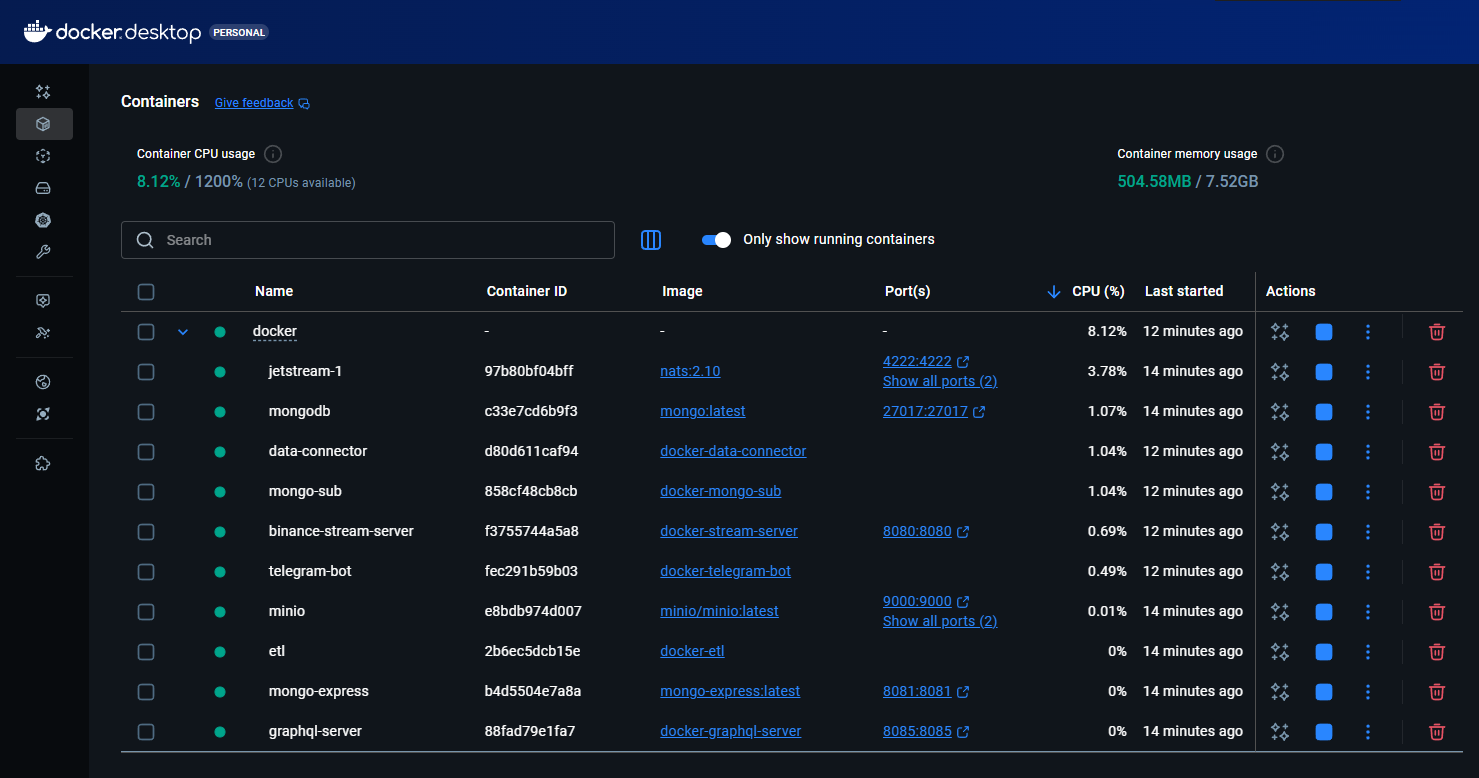
\includegraphics[width=0.85\textwidth,keepaspectratio]{rysunki/docker_desktop}
    \caption{Zestawienie aktywnych usług wchodzących w skład projektowanego systemu w środowisku Docker.}
    \label{fig:docker_desktop}
\end{figure}

\subsection{NATS JetStream}
\label{subsec:tech_nats}

NATS JetStream to rozproszony broker wiadomości zaprojektowany z~myślą o~wysokiej wydajności i~niskim opóźnieniu.
W~porównaniu do alternatyw takich jak Apache Kafka czy RabbitMQ, JetStream charakteryzuje się prostszą konfiguracją,
mniejszymi wymaganiami zasobowymi oraz natywnym wsparciem dla semantyki \textit{at-least-once} bez konieczności
zewnętrznej bazy danych~\cite{nats_jetstream_docs_persistence_at_least_once}.

NATS jest szczególnie odpowiedni dla scenariuszy wymagających niskich opóźnień, takich jak przetwarzanie danych
finansowych w~czasie rzeczywistym~\cite{time_value_curve}.

\subsection{MongoDB}
\label{subsec:tech_mongodb}

MongoDB to dokumentowa baza danych NoSQL, która zapewnia elastyczność schematu oraz wysoką wydajność zapisów~\cite{mongodb_manual}.
W~kontekście projektu, kluczowe zalety to:
\begin{itemize}
    \item Natywna obsługa dokumentów JSON, co eliminuje konieczność mapowania obiektowo-relacyjnego.
    \item Bogate możliwości agregacji danych (Aggregation Framework).
    \item Łatwa integracja z~językiem Go poprzez oficjalny sterownik.
\end{itemize}

W systemie MongoDB pełni rolę warstwy gorącej (\textit{hot storage}) przeznaczonej do szybkiego zapisu zdarzeń oraz
obsługi zapytań o~najnowsze dane.
Rysunki~\ref{fig:mongo_trade_record} oraz~\ref{fig:mongo_notification} przedstawiają strukturę kolekcji
oraz przykładowe rekordy.

\begin{figure}[H]
    \centering
    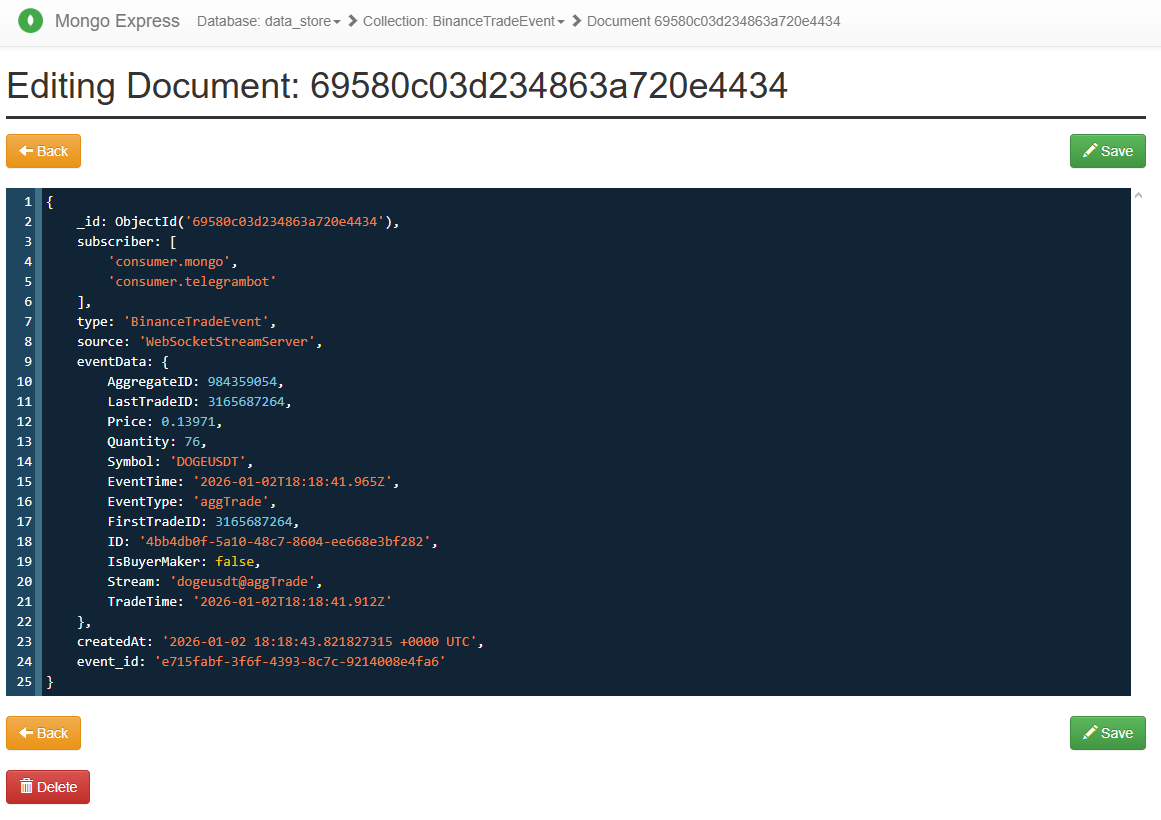
\includegraphics[width=0.85\textwidth,keepaspectratio]{rysunki/mongo_trade_record}
    \caption{Przykładowy rekord w~kolekcji BinanceTradeEvent zawierający pola domenowe transakcji oraz metadane.}
    \label{fig:mongo_trade_record}
\end{figure}

\begin{figure}[H]
    \centering
    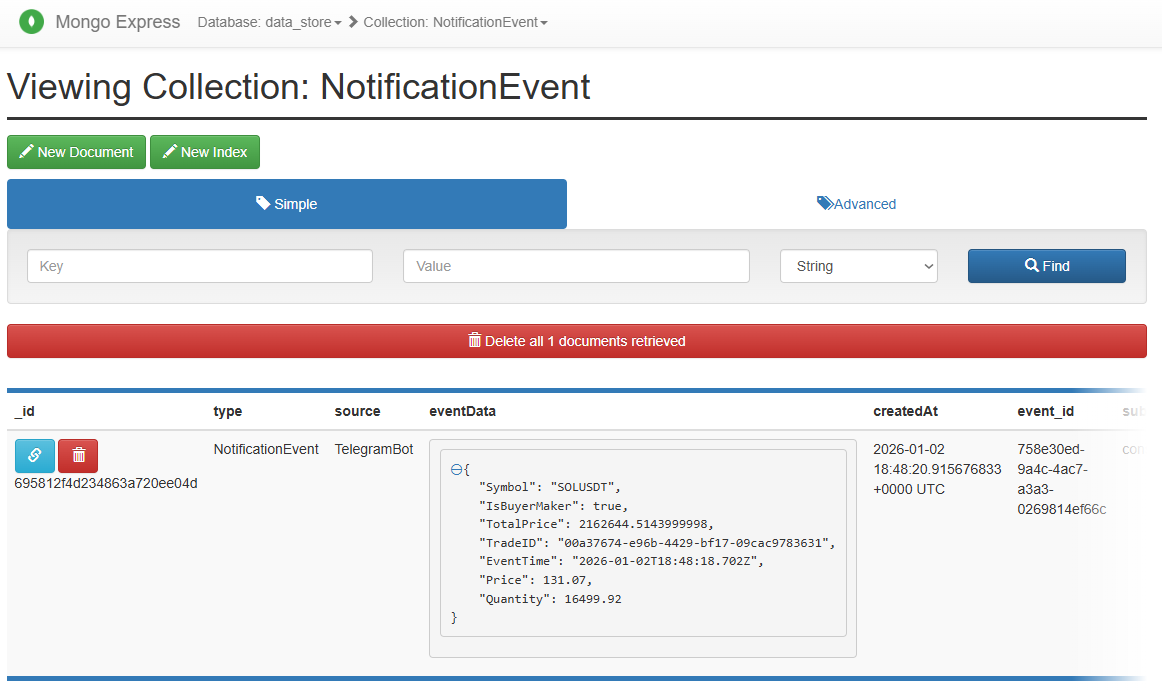
\includegraphics[width=0.85\textwidth,keepaspectratio]{rysunki/mongo_notification}
    \caption{Kolekcja NotificationEvent w~MongoDB przechowująca zdarzenia generowane przez system.}
    \label{fig:mongo_notification}
\end{figure}

\subsection{MinIO}
\label{subsec:tech_minio}

MinIO to wysokowydajny magazyn obiektowy kompatybilny z~protokołem Amazon S3.
Wybór MinIO podyktowany był możliwością uruchomienia w~środowisku lokalnym (\textit{on-premises}) bez zależności od
chmury publicznej, co jest kluczowe dla założeń projektu~\cite{cloud_repatriation_researchgate}.
MinIO zapewnia funkcje korporacyjne takie jak wersjonowanie, szyfrowanie i~replikacja, przy zachowaniu prostoty
wdrożenia w~kontenerze Docker~\cite{minio_docs}.

W ramach systemu MinIO pełni rolę warstwy zimnej (\textit{cold storage}) dla danych historycznych oraz warstwy
analitycznej.
Dane w~bucketach są organizowane w~sposób wspierający zarówno przetwarzanie przyrostowe, jak i~zapytania wsadowe.
Dla danych surowych zastosowano hierarchię katalogów według czasu (rok/miesiąc/dzień/godzina), natomiast dla danych
przetworzonych i~agregatów wykorzystano partycjonowanie w~stylu
klucz-wartość (np.\ symbol=DOGEUSDT/date=2025-12-05) w celu optymalizacji zapytań~\cite{hive_partitioning}.
Rysunki od~\ref{fig:minio_homepage} oraz~\ref{fig:minio_analytics_example} ilustrują zawartość bucketa binance-trades
w~MinIO oraz przykładową zawartość pliku z~agregatami czasowymi.

\begin{figure}[H]
    \centering
    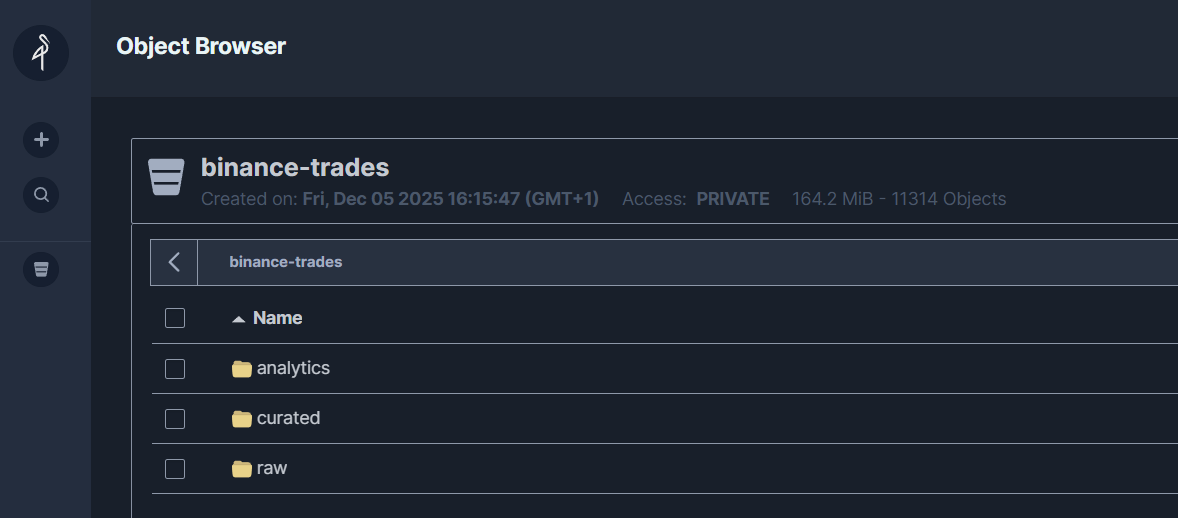
\includegraphics[width=0.85\textwidth,keepaspectratio]{rysunki/minio_homepage}
    \caption{Widok bucketa binance-trades w~MinIO z~podziałem na warstwy: raw (dane surowe), curated (dane
    oczyszczone) oraz analytics (agregaty).}
    \label{fig:minio_homepage}
\end{figure}

\begin{figure}[H]
    \centering
    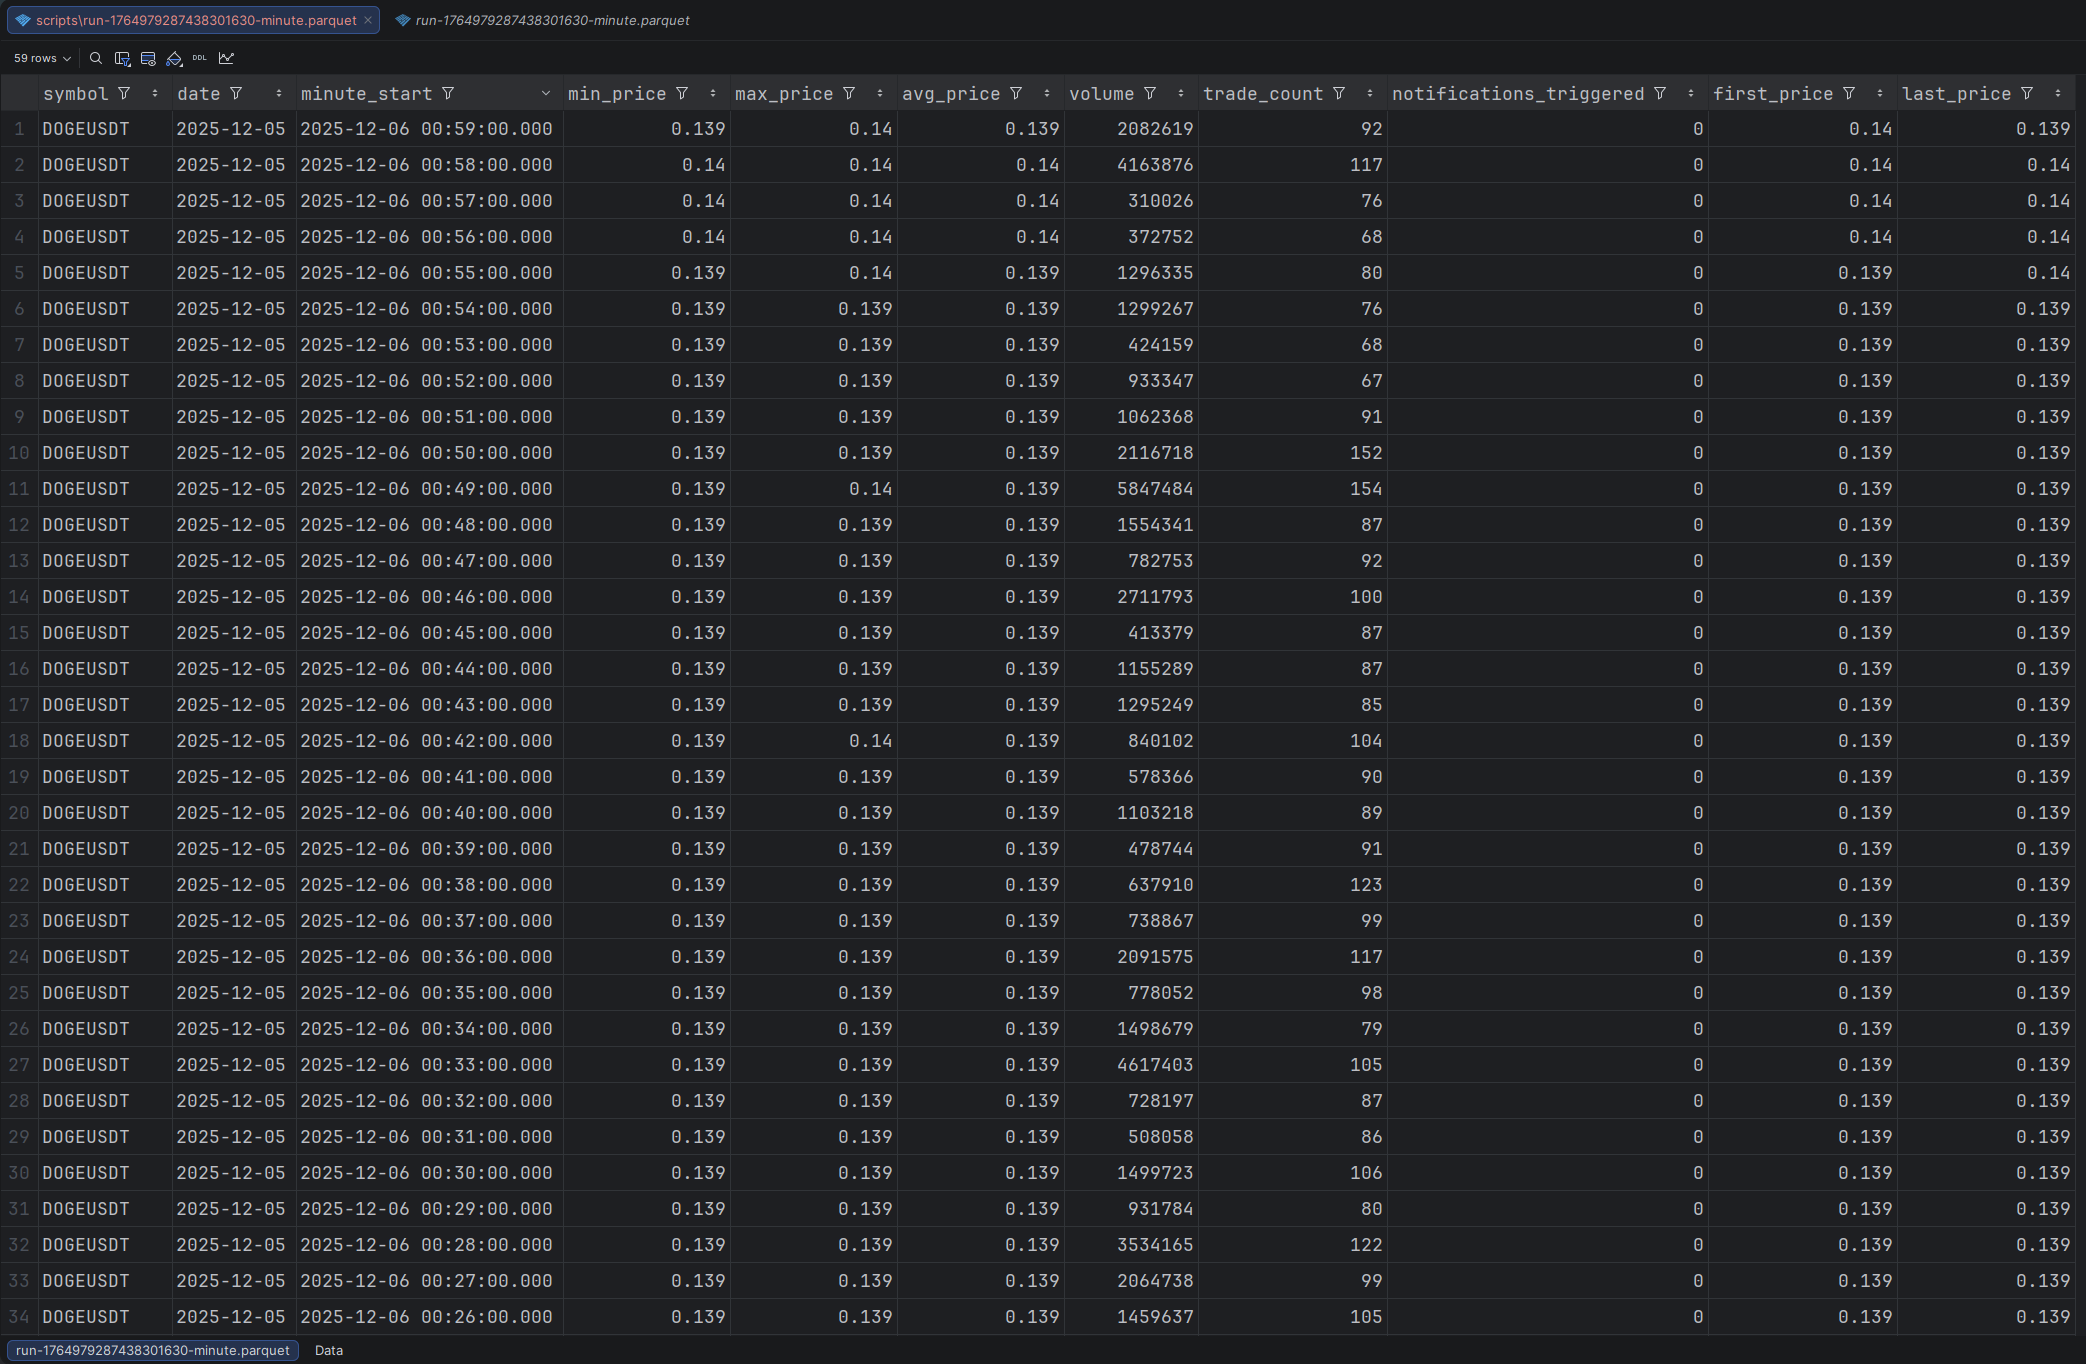
\includegraphics[width=0.85\textwidth,keepaspectratio]{rysunki/minio_analytics_example}
    \caption{Przykładowa zawartość pliku z~agregatami minutowymi w~warstwie analytics.}
    \label{fig:minio_analytics_example}
\end{figure}

\subsection[GraphQL i gqlgen]{GraphQL i~gqlgen}
\label{subsec:tech_graphql}

GraphQL to język zapytań do interfejsów API, który umożliwia klientom precyzyjne definiowanie struktury odpowiedzi.
Biblioteka gqlgen generuje typowany kod Go na podstawie schematu GraphQL, zapewniając spójność typów
w~czasie kompilacji oraz wysoką wydajność dzięki unikaniu refleksji w~czasie wykonania~\cite{graphql_docs}.

Schemat GraphQL zapisywany jest w~postaci SDL (\textit{Schema Definition Language}), czyli deklaratywnej definicji
obiektów domenowych, typów wejściowych (\textit{input}) oraz dostępnych operacji (\textit{query}).
W~SDL znak wykrzyknika oznacza pole wymagane (\textit{non-null}), tzn.\ serwer gwarantuje, że wartość nie
będzie pusta.
Z~kolei nawiasy kwadratowe oznaczają listę elementów~\cite{gqlgen_docs}.

Poniższy zrzut ekranu (Rysunek~\ref{fig:gql_query_example_0}) przedstawia przykładowe zapytanie GraphQL, które ilustruje
elastyczność API w~zakresie doboru pól oraz warunków filtrowania.

\begin{figure}[H]
    \centering
    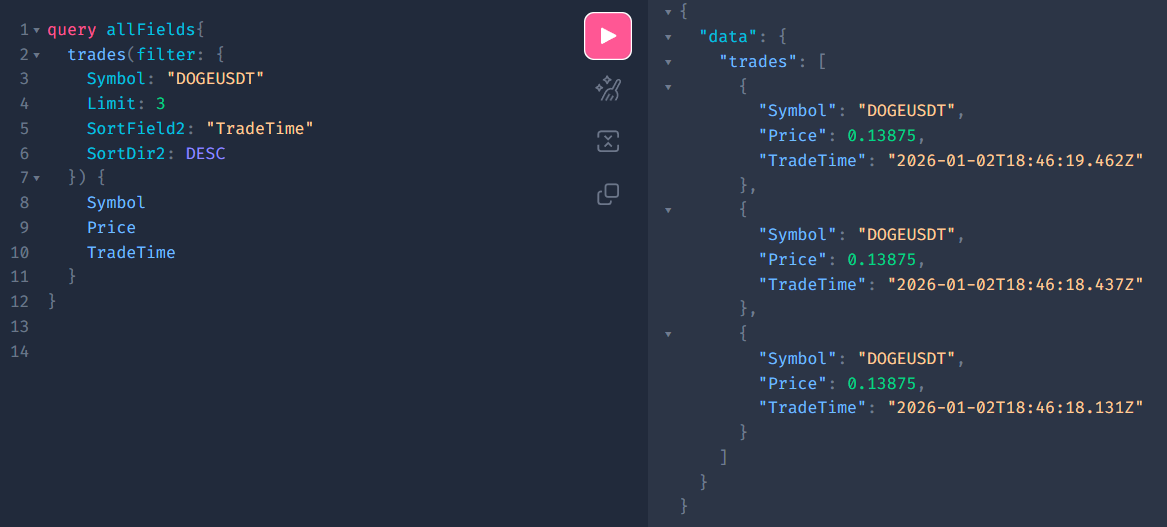
\includegraphics[width=0.85\textwidth,keepaspectratio]{rysunki/gql_query_example_0}
    \caption{Przykładowe zapytanie: trzy najnowsze zdarzenia dla symbolu DOGEUSDT\@.}
    \label{fig:gql_query_example_0}
\end{figure}

\subsection[Modele danych w języku Go]{Modele danych w~języku Go}
\label{subsec:tech_models}

Warstwa modeli w~języku Go opisuje struktury danych wykorzystywane na kolejnych etapach potoku: od~danych wejściowych
z~WebSocket, przez zdarzenia zapisywane w~bazie, aż po~dane przygotowane do archiwizacji w~magazynie obiektowym.
Jawne typy struktur stanowią kontrakt między mikroserwisami oraz ograniczają liczbę błędów integracyjnych dzięki
weryfikacji typów w~czasie kompilacji.
Rysunek~\ref{fig:model_data} przedstawia strukturę (\textit{BinanceTradeData}) wykorzystywaną do~reprezentacji danych
odebranych z~WebSocket.

\begin{figure}[H]
    \centering
    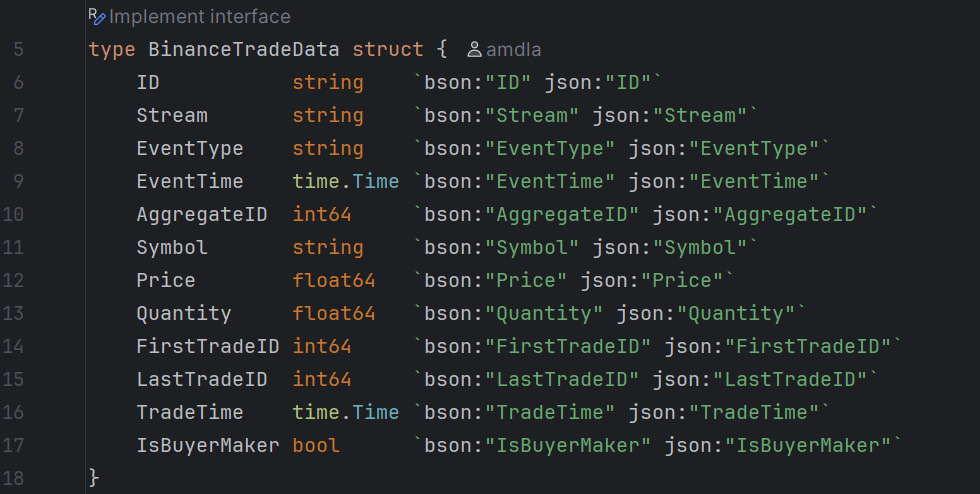
\includegraphics[width=0.65\textwidth,keepaspectratio]{rysunki/model_data}
    \caption{Struktura BinanceTradeData --- podstawowy model danych transakcyjnych pobierany z~WebSocket.}
    \label{fig:model_data}
\end{figure}

\subsection{Format Parquet}
\label{subsec:tech_parquet}

Apache Parquet to kolumnowy format przechowywania danych, zoptymalizowany pod kątem analitycznych obciążeń odczytu.
Kluczowe zalety~\cite{apache_parquet_docs}:
\begin{itemize}
    \item Efektywna kompresja kolumnowa (często 10x redukcja rozmiaru względem JSON).
    \item Szybkie odczyty selektywne (tylko wybrane kolumny są dekompresowane).
    \item Wsparcie dla złożonych schematów z~zagnieżdżonymi strukturami.
    \item Szeroka kompatybilność z~narzędziami analitycznymi (Pandas, Spark, DuckDB).
\end{itemize}

\subsection{Viper}
\label{subsec:tech_viper}

Viper to biblioteka Go do zarządzania konfiguracją, wspierająca wiele źródeł z~możliwością hierarchicznego
nadpisywania.
Umożliwia elastyczne konfigurowanie mikroserwisów bez konieczności rekompilacji~\cite{viper_lib}.

\subsection[Jupyter Notebook i Python]{Jupyter Notebook i~Python}
\label{subsec:tech_jupyter}

Jupyter Notebook służy jako interfejs do eksploracyjnej analizy danych historycznych przechowywanych w~MinIO\@.
Środowisko Python z~bibliotekami Pandas, PyArrow i~scikit-learn umożliwia~\cite{jupyter_docs}:
\begin{itemize}
    \item Interaktywną eksplorację zbiorów danych.
    \item Wizualizację trendów i~anomalii.
    \item Prototypowanie modeli uczenia maszynowego.
    \item Generowanie raportów analitycznych.
\end{itemize}


\section[Problemy i wyzwania]{Problemy i~wyzwania}
\label{sec:problemy_wyzwania}

Realizacja systemu o~architekturze rozproszonej wiąże się z~szeregiem wyzwań projektowych i~implementacyjnych,
które wymagają świadomych kompromisów oraz zastosowania odpowiednich wzorców i~praktyk inżynierskich.
Poniżej przedstawiono kluczowe problemy zidentyfikowane w~trakcie projektowania i~implementacji systemu.

\subsection{Złożoność architektury mikrousługowej}
\label{subsec:zlozonosc_mikrouslug}

Architektura mikrousługowa, pomimo licznych zalet takich jak niezależne skalowanie i~wdrażanie, wprowadza znaczącą
złożoność operacyjną.
Każdy mikroserwis wymaga własnej konfiguracji, zarządzania zależnościami, obsługi błędów oraz monitorowania.
Liczba potencjalnych punktów awarii rośnie proporcjonalnie do liczby komponentów, co wymaga wdrożenia strategii
odporności (\textit{resilience patterns}).

Komunikacja między serwisami poprzez sieć wprowadza dodatkowe źródła opóźnień i~błędów (timeouty, utrata połączenia,
przeciążenie), które muszą być obsługiwane na poziomie aplikacji.
W~tradycyjnych systemach monolitycznych, wywołania między modułami realizowane są w~ramach jednego procesu, co
eliminuje tę klasę problemów~\cite{newman_building_microservices}.

\subsection[Debugowanie i śledzenie rozproszone]{Debugowanie i~śledzenie rozproszone}
\label{subsec:debugowanie}

Diagnostyka problemów w~systemie rozproszonym jest znacząco bardziej złożona niż w~aplikacji monolitycznej.
Pojedyncze żądanie użytkownika może przepływać przez wiele usług, a~logi każdej z~nich muszą zostać skorelowane
w~celu odtworzenia pełnego obrazu sytuacji.
Wymaga to implementacji mechanizmów propagacji kontekstu (np.\ identyfikatorów korelacji) oraz centralizacji logów.

Dodatkowo, błędy związane z~kolejnością zdarzeń są trudniejsze do reprodukcji w~środowisku rozproszonym, gdzie czas
wykonania poszczególnych operacji zależy od wielu czynników zewnętrznych~\cite{open_telemetry}.

\subsection{Przetwarzanie sterowane zdarzeniami}
\label{subsec:event_driven_challenges}

Paradygmat \textit{Event-Driven Architecture} wymaga odmiennego podejścia do projektowania niż tradycyjne systemy
oparte na synchronicznych wywołaniach.
Należy precyzyjnie zdefiniować strukturę zdarzeń (kontrakty), zapewnić wersjonowanie schematów oraz obsłużyć
scenariusze takie jak zdarzenia niespójne czasowo (\textit{out-of-order events}) czy zduplikowane komunikaty~\cite{at_least_once}.

\subsection{Zarządzanie wieloma kontenerami}
\label{subsec:zarzadzanie_kontenerami}

System składa się z~wielu kontenerów Docker, których uruchomienie i~koordynacja wymaga odpowiedniej konfiguracji
orkiestracji.
Proces uruchamiania pełnego środowiska deweloperskiego jest czasochłonny (kilka minut), co wydłuża cykl
debugowania --- nawet drobna literówka w~kodzie wymaga przebudowania obrazu i~restartu kontenera.

Ponadto, duża liczba kontenerów i~wolumen przetwarzanych danych przekładają się na znaczące wymagania zasobowe.
Optymalizacja wykorzystania pamięci i~procesora jest niezbędna do uruchomienia systemu na typowej stacji roboczej
dewelopera.

\subsection[Jednoczesny dostęp do danych historycznych i bieżących]{Jednoczesny dostęp do danych historycznych i~bieżących}
\label{subsec:dostep_danych}

Specyficznym wyzwaniem jest zapewnienie jednoczesnego dostępu do danych w~dwóch warstwach o~odmiennych
charakterystykach.
Warstwa gorąca (MongoDB) optymalizowana jest pod kątem szybkich zapisów i~zapytań punktowych, natomiast warstwa
zimna (MinIO) przeznaczona jest do sekwencyjnego odczytu dużych zbiorów danych.

\subsection{Projektowanie elastycznego API}
\label{subsec:projektowanie_api}

Zaprojektowanie interfejsu GraphQL umożliwiającego elastyczne zapytania z~wieloma filtrami wymagało głębokiego
zrozumienia specyfiki tego standardu.
GraphQL różni się znacząco od REST pod względem modelowania danych, obsługi błędów oraz optymalizacji wydajności~\cite{graphql_docs}.

Dodatkowo, biblioteka gqlgen wymaga zdefiniowania schematu w~języku SDL (\textit{Schema Definition Language}),
a~następnie implementacji (\textit{resolverów}) --- funkcji odpowiedzialnych za pobieranie danych dla poszczególnych pól~\cite{gqlgen_docs}.

\subsection{Optymalizacja procesu archiwizacji}
\label{subsec:optymalizacja_archiwizacji}

Efektywne przenoszenie danych między warstwami wymaga starannej optymalizacji pod kątem wykorzystania zasobów
sieciowych i~dyskowych.
Proces musi być realizowany przyrostowo, bez blokowania bieżących operacji, z~mechanizmem wznawiania w~przypadku
przerwania.

Kompresja danych do formatu Parquet jest operacją kosztowną obliczeniowo, dlatego należy wyważyć stopień kompresji
(a~co za tym idzie oszczędność miejsca) z~czasem wykonania procesu archiwizacji.


    \section{Możliwości dalszego rozwoju}
\label{sec:rozwoj}

Wdrożony system stanowi działający \textit{proof of concept} architektury do przetwarzania i~archiwizacji danych
rynkowych w~czasie rzeczywistym w~środowisku \textit{on-premises}.
Z~uwagi na mikrousługowy charakter rozwiązania oraz silnie operacyjny kontekst przetwarzania strumieniowego,
istnieje szereg naturalnych kierunków rozwoju, które pozwoliłyby zwiększyć niezawodność, ułatwić diagnozę
problemów oraz rozszerzyć funkcjonalność analityczną.
Poniżej przedstawiono wybrane propozycje.

\subsection{Centralizacja logów}

W~obecnej postaci każdy mikroserwis zapisuje logi niezależnie, co utrudnia szybkie odtworzenie przebiegu zdarzeń
w~sytuacji awarii lub rozbieżności danych.
Wprowadzenie centralizacji logów (np.\ poprzez standaryzację logów w~formacie JSON, dodanie identyfikatora korelacji
oraz wysyłkę do wspólnego backendu typu Loki/ELK) umożliwiłoby analizę całego systemu w~jednym miejscu.
Taka zmiana skraca czas diagnostyki oraz ułatwia analizę zależności między komponentami.

\subsection[Metryki i dashboardy (Prometheus/Grafana)]{Metryki i~dashboardy (Prometheus/Grafana)}

Kolejnym krokiem jest ekspozycja metryk technicznych i~domenowych, takich jak: opóźnienie od odbioru zdarzenia do
zapisania w~bazie, procent błędów walidacji, opóźnienie konsumentów JetStream, czasy odpowiedzi API GraphQL czy wydajność
procesów archiwizacji.
Wysyłanie tych metryk do systemu typu Prometheus oraz budowa dashboardów w~Grafanie pozwoliłaby nie tylko
monitorować bieżący stan, ale również planować zasoby na podstawie trendów i~wykrywać degradację wydajności zanim
stanie się odczuwalna dla użytkownika~\cite{prometheus_grafana}.

\subsection{Śledzenie rozproszone (distributed tracing)}

W~systemie sterowanym zdarzeniami pojedyncze zdarzenie przechodzi przez wiele komponentów, co utrudnia śledzenie jego
przebiegu.
Wdrożenie śledzenia rozproszonego (np.\ OpenTelemetry) wraz z~propagacją kontekstu (\texttt{trace\_id}) między
mikroserwisami pozwoliłoby na wizualizację pełnej ścieżki przetwarzania i~precyzyjne wskazanie wąskich gardeł~\cite{open_telemetry}.
Jest to szczególnie istotne przy skalowaniu systemu oraz przy analizie incydentów trudnych do odtworzenia.

\subsection[Alerty operacyjne i powiadomienia o stanie systemu]{Alerty operacyjne i~powiadomienia o~stanie systemu}

W~projekcie istnieje bot Telegram wykorzystywany do powiadomień o~zdarzeniach rynkowych.
Naturalnym rozszerzeniem jest dodanie warstwy alertów operacyjnych, które informowałyby o~problemach działania
systemu: braku nowych danych, wysokim poziomie błędów, rosnącym opóźnieniu konsumentów, przekroczeniu progów
zużycia zasobów czy nieudanych migracjach danych do MinIO\@.
Alerty oparte o~metryki i~logi pozwoliłyby reagować szybciej i~skrócić czas przestojów.

\subsection[Rozszerzenie API: dostęp do danych z MinIO oraz federacja GraphQL]{Rozszerzenie API: dostęp do danych z~MinIO oraz federacja GraphQL}

Obecne API GraphQL udostępnia dane z~warstwy gorącej (MongoDB).
Dodanie zapytań do danych historycznych i~analitycznych przechowywanych w~MinIO umożliwiłoby obsługę szerszego
zakresu przypadków użycia, takich jak pobieranie agregatów, dłuższych okien czasowych oraz danych do treningu
modeli.

W~praktyce wygodnym podejściem jest zastosowanie federacji GraphQL, czyli mechanizmu pozwalającego łączyć wiele
niezależnych schematów i~serwerów GraphQL w~jeden spójny endpoint.
Federacja działa jak \textit{GraphQL dla endpointów GraphQL}: klient widzi jedno API pod jednym adresem, natomiast bramka
\textit{gateway} rozdziela zapytania do właściwych podserwisów i~składa odpowiedź w~całość~\cite{apollo_federation_architecture}.
Takie rozwiązanie upraszcza rozwój i~wdrażanie, ponieważ poszczególne części API mogą ewoluować niezależnie.

\subsection{Bardziej zaawansowany moduł analityczny}

Aktualna warstwa analityczna ma charakter demonstracyjny i~koncentruje się na podstawowej agregacji.
Kolejnym krokiem mogłoby być rozszerzenie zakresu obliczeń o~cechy realnie wykorzystywane w~analizie
ilościowej, takie jak zmienność w~oknach kroczących, miary trendu i~momentum, wykrywanie anomalii czy proste
sygnały zdarzeniowe.

\subsection[Modele predykcyjne i pipeline uczenia maszynowego]{Modele predykcyjne i~pipeline uczenia maszynowego}

System dostarcza obecnie dane oczyszczone i~zagregowane, co stanowi dobry fundament do budowy modeli predykcyjnych.
Dalszy rozwój mógłby obejmować przygotowanie pełnego potoku ML: definicję etykiet, walidację czasową,
rejestrowanie eksperymentów oraz wersjonowanie modeli.
W~wariancie produkcyjnym można rozważyć osobny serwis publikujący predykcje jako kolejne zdarzenia w
NATS, co pozwoliłoby wykorzystywać je w~powiadomieniach lub dalszych procesach ETL\@.

\subsection[Dalsza optymalizacja i skalowanie do wszystkich symboli]{Dalsza optymalizacja i~skalowanie do wszystkich symboli}

Aktualnie system obsługuje ograniczoną liczbę symboli, co upraszcza przetwarzanie i~zmniejsza wymagania zasobowe.
Skalowanie do pełnej listy symboli dostępnych na giełdzie wymagałoby poprawy mechanizmów \textit{backpressure},
fragmentacji strumieni i~konsumentów (np.\ podział po symbolu lub klasie instrumentów), grupowania zapisów do baz oraz
lepszego ograniczania kosztów obliczeniowych w~ETL\@.
Taki kierunek rozwoju jest istotny, jeśli celem systemu miałoby być pełne odwzorowanie rynku w~czasie rzeczywistym.

    \chapter{Weryfikacja rozwiązania}
\label{ch:testy}

W~celu weryfikacji poprawności działania zaprojektowanego systemu przeprowadzono serię testów manualnych obejmujących
wszystkie kluczowe komponenty architektury.
Testy miały na celu potwierdzenie, że każdy z~mikroserwisów realizuje przypisane mu funkcje zgodnie z~założeniami
przedstawionymi w~rozdziałach~\ref{ch:analiza} i~\ref{ch:projekt}.

Scenariusze testowe skupiały się na weryfikacji następujących aspektów systemu:
\begin{itemize}
    \item Poprawność połączenia z~zewnętrznymi źródłami danych (WebSocket Binance) oraz odbierania strumieniowych
    zdarzeń rynkowych.
    \item Funkcjonowanie magistrali komunikacyjnej NATS JetStream, w~tym publikowanie i~subskrybowanie zdarzeń przez
    poszczególne komponenty.
    \item Działanie systemu powiadomień Telegram oraz modułu zapisu do bazy MongoDB\@.
    \item Działanie mechanizmu filtrowania powiadomień w~zależności od parametrów zdarzeń.
    \item Poprawność zapytań GraphQL z~różnymi filtrami, zarówno zwracającymi wyniki, jak i~pustymi zbiorami danych.
    \item Proces ETL oraz mechanizm \textit{tiered storage}, obejmujący przenoszenie danych z~warstwy gorącej
    (MongoDB) do warstwy zimnej (MinIO) oraz tworzenie zbiorów danych w~formacie Parquet.
\end{itemize}

Każdy test został przeprowadzony w~środowisku Docker z~wykorzystaniem obrazów zbudowanych na podstawie kodu źródłowego
projektu.
Wszystkie scenariusze zakończyły się wynikiem pozytywnym, potwierdzając tym samym zgodność implementacji z~założeniami
projektowymi.

Poniżej przedstawiono szczegółowe opisy poszczególnych scenariuszy testowych.


\newpage


\section[Test T1: Odbiór danych z Binance WebSocket]{Test T1: Odbiór danych z~Binance WebSocket}
\label{sec:test_binance_websocket}

Test weryfikuje poprawność połączenia serwera strumieniowego z~API Binance oraz odbierania komunikatów WebSocket
zawierających zdarzenia typu \textit{aggTrade}.

\vspace{0.5cm}

\begin{table}[H]
    \centering
    \caption{Scenariusz testowy T1: Odbiór danych z~Binance WebSocket.}
    \label{tab:test_binance_websocket}
    \begin{tabular}{|p{0.25\textwidth}|p{0.65\textwidth}|}
        \hline
        \textbf{Pole}        & \textbf{Treść}                                                                                                                                                                                                                                      \\ \hline
        Nazwa scenariusza    & Odbiór danych rynkowych z~Binance WebSocket                                                                                                                                                                                                         \\ \hline
        Cel testu            & Weryfikacja poprawności nawiązania połączenia WebSocket z~API Binance oraz odbierania strumieniowych zdarzeń transakcyjnych dla wybranych par handlowych                                                                                            \\ \hline
        Parametry testu      & Lista symboli: \textit{BTCUSDT, ETHUSDT}; URL WebSocket: \textit{wss://fstream.binance.com/stream?streams=} \newline \textit{btcusdt@aggTrade/ethusdt@aggTrade}                                                                                     \\ \hline
        Kroki testowe        & 1. Uruchomienie kontenera \textit{stream\_server}. \newline 2. Nawiązanie połączenia z~endpointem Binance WebSocket. \newline 3. Nasłuchiwanie wiadomości przychodzących. \newline 4. Analiza logów aplikacji w~celu potwierdzenia odbioru zdarzeń. \\ \hline
        Oczekiwany rezultat  & Aplikacja nawiązuje połączenie WebSocket, odbiera komunikaty w~formacie JSON zawierające pola: \textit{stream}, \textit{data} (z~zagnieżdżonymi polami \textit{e, E, s, p, q, T, m}), oraz loguje odbiór zdarzeń.                                   \\ \hline
        Rzeczywisty rezultat & Połączenie zostało nawiązane poprawnie. Aplikacja otrzymała komunikaty JSON zgodne z~dokumentacją Binance, w~logach pojawiły się wpisy potwierdzające odbiór zdarzeń typu \textit{aggTrade}.                                                        \\ \hline
    \end{tabular}
\end{table}

Test potwierdził, że serwer strumieniowy poprawnie nawiązuje połączenie z~API Binance oraz odbiera dane rynkowe
w~czasie rzeczywistym.
Otrzymane komunikaty zawierały wszystkie wymagane pola domenowe (symbol, cena, wolumen, znacznik czasowy), co
umożliwiło dalsze przetwarzanie zdarzeń przez system.

\newpage


\section{Test T2: Publikowanie zdarzeń do NATS JetStream}
\label{sec:test_nats_publish}

Test weryfikuje poprawność publikowania odebranych zdarzeń z~Binance do magistrali komunikacyjnej NATS JetStream oraz
ich dostępność w~kolejce dla innych konsumentów.

\vspace{0.5cm}

\begin{table}[H]
    \centering
    \caption{Scenariusz testowy T2: Publikowanie zdarzeń do NATS JetStream.}
    \label{tab:test_nats_publish}
    \begin{tabular}{|p{0.25\textwidth}|p{0.65\textwidth}|}
        \hline
        \textbf{Pole}        & \textbf{Treść}                                                                                                                                                                                                                                                                        \\ \hline
        Nazwa scenariusza    & Publikowanie zdarzeń do kolejki NATS JetStream                                                                                                                                                                                                                                        \\ \hline
        Cel testu            & Weryfikacja poprawności publikowania zdarzeń typu \textit{BinanceTradeEvent} do strumienia NATS oraz ich trwałego zapisu w~kolejce                                                                                                                                                    \\ \hline
        Parametry testu      & Stream: \textit{EVENTS}, Subject: \textit{input.events}, Typ zdarzenia: \textit{BinanceTradeEvent} zawierający pola: \textit{ID, Subscribers, Type, Source, EventData, CreatedAt}                                                                                                     \\ \hline
        Kroki testowe        & 1. Uruchomienie serwera strumieniowego oraz NATS JetStream. \newline 2. Odebranie komunikatu z~Binance WebSocket. \newline 3. Opakowanie danych w~strukturę \textit{Event} i~publikacja do kolejki. \newline 4. Weryfikacja obecności zdarzenia w~streamie za pomocą logów aplikacji. \\ \hline
        Oczekiwany rezultat  & Zdarzenie zostaje poprawnie opublikowane do strumienia \textit{EVENTS} na subject \textit{input.events}. W~logach pojawia się wpis potwierdzający publikację wraz z~identyfikatorem zdarzenia. Zdarzenie jest dostępne dla konsumentów subskrybujących dany strumień.                 \\ \hline
        Rzeczywisty rezultat & Zdarzenie zostało pomyślnie opublikowane do NATS JetStream. Logi aplikacji potwierdziły publikację z~odpowiednim identyfikatorem UUID\@. Zdarzenie znalazło się w~kolejce i~jest dostępne dla konsumentów.                                                                            \\ \hline
    \end{tabular}
\end{table}

Test potwierdził poprawne działanie mechanizmu publikowania zdarzeń do magistrali NATS JetStream.
Serwer strumieniowy przekształca surowe komunikaty z~WebSocket w~strukturę \textit{Event} zawierającą metadane (typ,
źródło, lista subskrybentów), a~następnie publikuje je do kolejki.

\newpage


\section{Test T3: Subskrybowanie zdarzeń przez moduł MongoDB}
\label{sec:test_mongo_subscribe}

Test weryfikuje poprawność subskrybowania zdarzeń z~kolejki NATS JetStream przez moduł MongoDB oraz zapisywania ich do
odpowiednich kolekcji.

\vspace{0.5cm}

\begin{table}[H]
    \centering
    \caption{Scenariusz testowy T3: Subskrybowanie zdarzeń przez moduł MongoDB.}
    \label{tab:test_mongo_subscribe}
    \begin{tabular}{|p{0.25\textwidth}|p{0.65\textwidth}|}
        \hline
        \textbf{Pole}        & \textbf{Treść}                                                                                                                                                                                                                                                                                           \\ \hline
        Nazwa scenariusza    & Odbiór zdarzeń przez konsument MongoDB                                                                                                                                                                                                                                                                   \\ \hline
        Cel testu            & Weryfikacja poprawności subskrybowania zdarzeń z~kolejki NATS oraz zapisywania ich do bazy MongoDB w~odpowiedniej kolekcji                                                                                                                                                                               \\ \hline
        Parametry testu      & Subject: \textit{consumer.mongo}, Durable: \textit{mongo-subscriber-durable}, Typ zdarzenia: \textit{BinanceTradeEvent}, Kolekcja docelowa: \textit{BinanceTradeEvent}                                                                                                                                   \\ \hline
        Kroki testowe        & 1. Uruchomienie kontenerów NATS oraz MongoDB. \newline 2. Publikacja zdarzenia do kolejki NATS na subject \textit{consumer.mongo}. \newline 3. Oczekiwanie na przetworzenie zdarzenia przez konsumenta. \newline 4. Weryfikacja obecności rekordu w~bazie MongoDB w~kolekcji \textit{BinanceTradeEvent}. \\ \hline
        Oczekiwany rezultat  & Konsument MongoDB odbiera zdarzenie z~kolejki NATS, wyodrębnia pola: \textit{event\_id, subscriber, type, source, eventData, createdAt}, tworzy dokument BSON i~zapisuje go do kolekcji. W~logach pojawia się wpis potwierdzający zapis z~identyfikatorem zdarzenia.                                     \\ \hline
        Rzeczywisty rezultat & Zdarzenie zostało odebrane i~przetworzone poprawnie. Dokument z~odpowiednimi polami został zapisany do kolekcji \textit{BinanceTradeEvent}. Logi potwierdziły operację z~identyfikatorem zdarzenia.                                                                                                      \\ \hline
    \end{tabular}
\end{table}

Test potwierdził poprawne działanie konsumenta MongoDB jako subskrybenta zdarzeń z~magistrali NATS\@.
Moduł poprawnie odbiera komunikaty, deserializuje je z~formatu JSON do struktury \textit{Event}, konwertuje na
dokumenty BSON oraz zapisuje do odpowiednich kolekcji na podstawie pola \textit{type}.

\newpage


\section{Test T4: Subskrybowanie zdarzeń przez moduł Telegram Bot}
\label{sec:test_telegram_subscribe}

Test weryfikuje poprawność subskrybowania zdarzeń z~kolejki NATS JetStream przez moduł Telegram Bot oraz przetwarzania
komunikatów w~celu wysyłania powiadomień.

\vspace{0.5cm}

\begin{table}[H]
    \centering
    \caption{Scenariusz testowy T4: Subskrybowanie zdarzeń przez moduł Telegram Bot.}
    \label{tab:test_telegram_subscribe}
    \begin{tabular}{|p{0.25\textwidth}|p{0.65\textwidth}|}
        \hline
        \textbf{Pole}        & \textbf{Treść}                                                                                                                                                                                                                                                                                                          \\ \hline
        Nazwa scenariusza    & Odbiór zdarzeń przez konsument Telegram Bot                                                                                                                                                                                                                                                                             \\ \hline
        Cel testu            & Weryfikacja poprawności subskrybowania zdarzeń z~kolejki NATS przez moduł Telegram Bot oraz przetwarzania komunikatów                                                                                                                                                                                                   \\ \hline
        Parametry testu      & Subject: \textit{consumer.telegrambot}, Durable: \textit{telegram-bot-durable}, Typ zdarzenia: \textit{BinanceTradeEvent}                                                                                                                                                                                               \\ \hline
        Kroki testowe        & 1. Uruchomienie kontenerów NATS oraz \textit{telegram\_bot}. \newline 2. Publikacja zdarzenia do kolejki NATS na subject \textit{consumer.telegrambot}. \newline 3. Oczekiwanie na przetworzenie zdarzenia przez konsument. \newline 4. Analiza logów aplikacji w~celu potwierdzenia odbioru i~przetworzenia zdarzenia. \\ \hline
        Oczekiwany rezultat  & Konsument Telegram Bot odbiera zdarzenie z~kolejki NATS, deserializuje je do struktury \textit{Event}, wyodrębnia dane \textit{BinanceTradeData} i~przetwarza je zgodnie z~logiką biznesową. W~logach pojawia się wpis potwierdzający odbiór zdarzenia.                                                                 \\ \hline
        Rzeczywisty rezultat & Zdarzenie zostało odebrane i~przetworzone poprawnie. Moduł Telegram Bot zdeserializował komunikat, wyodrębnił dane transakcji. Logi potwierdziły operację z~odpowiednim identyfikatorem zdarzenia.                                                                                                                      \\ \hline
    \end{tabular}
\end{table}

Test potwierdził poprawne działanie konsumenta Telegram Bot jako subskrybenta zdarzeń z~magistrali NATS\@.
Moduł poprawnie odbiera komunikaty oraz deserializuje zagnieżdżone dane typu \textit{BinanceTradeData} z~pola
\textit{EventData}, przygotowując je do dalszego przetwarzania przez mechanizm filtrowania.

\newpage


\section{Test T5: Wysyłanie powiadomienia Telegram -- filtr spełniony}
\label{sec:test_telegram_filter_pass}

Test weryfikuje poprawność działania mechanizmu filtrowania zdarzeń oraz wysyłania powiadomień przez Telegram Bot
w~przypadku spełnienia warunku filtra.

\vspace{0.5cm}

\begin{table}[H]
    \centering
    \caption{Scenariusz testowy T5: Wysyłanie powiadomienia Telegram -- filtr spełniony.}
    \label{tab:test_telegram_filter_pass}
    \begin{tabular}{|p{0.25\textwidth}|p{0.65\textwidth}|}
        \hline
        \textbf{Pole}        & \textbf{Treść}                                                                                                                                                                                                                                                                                                                                                       \\ \hline
        Nazwa scenariusza    & Wysyłanie powiadomienia przy spełnieniu warunku filtra                                                                                                                                                                                                                                                                                                               \\ \hline
        Cel testu            & Weryfikacja poprawności działania mechanizmu filtrowania oraz wysyłania powiadomień do Telegram w~przypadku, gdy wartość transakcji przekracza ustalony próg                                                                                                                                                                                                         \\ \hline
        Parametry testu      & Zdarzenie \textit{BinanceTradeEvent} z~polami: \textit{Price = 50000.0}, \textit{Quantity = 50.0}, wartość całkowita transakcji: 2~500~000 USD, próg filtra: 2~000~000 USD                                                                                                                                                                                           \\ \hline
        Kroki testowe        & 1. Publikacja zdarzenia do kolejki NATS na subject \textit{consumer.telegrambot}. \newline 2. Oczekiwanie na przetworzenie zdarzenia przez Telegram Bot. \newline 3. Weryfikacja warunku filtra (cena × ilość > 2~000~000). \newline 4. Sprawdzenie logów potwierdzających wysłanie powiadomienia. \newline 5. Weryfikacja otrzymania wiadomości na czacie Telegram. \\ \hline
        Oczekiwany rezultat  & Moduł Telegram Bot oblicza wartość całkowitą transakcji (50000.0 × 50.0 = 2~500~000), porównuje ją z~progiem 2~000~000 USD, stwierdza spełnienie warunku i~wysyła powiadomienie do Telegram API zawierające symbol, cenę, ilość oraz sformatowaną wartość całkowitą. W~logach pojawia się wpis o~wysłaniu alertu.                                                    \\ \hline
        Rzeczywisty rezultat & Warunek filtra został spełniony. Telegram Bot wysłał powiadomienie z~odpowiednimi danymi transakcji. Wiadomość została dostarczona na czat Telegram z~prawidłowo sformatowaną wartością całkowitą (2~500~000.00). Logi potwierdziły operację.                                                                                                                        \\ \hline
    \end{tabular}
\end{table}

Test potwierdził poprawne działanie mechanizmu filtrowania zdarzeń oraz integracji z~Telegram API\@.
System poprawnie oblicza wartość całkowitą transakcji, porównuje ją z~progiem zdefiniowanym w~funkcji
\textit{ValidateTrade} oraz wysyła powiadomienie w~formacie Markdown z~czytelnie sformatowaną kwotą.

\newpage


\section{Test T6: Brak powiadomienia Telegram -- filtr niespełniony}
\label{sec:test_telegram_filter_fail}

Test weryfikuje poprawność działania mechanizmu filtrowania w~przypadku, gdy zdarzenie nie spełnia warunku wysyłania
powiadomienia.

\vspace{0.5cm}

\begin{table}[H]
    \centering
    \caption{Scenariusz testowy T6: Brak powiadomienia Telegram -- filtr niespełniony.}
    \label{tab:test_telegram_filter_fail}
    \begin{tabular}{|p{0.25\textwidth}|p{0.65\textwidth}|}
        \hline
        \textbf{Pole}        & \textbf{Treść}                                                                                                                                                                                                                                                                                                                                                                                    \\ \hline
        Nazwa scenariusza    & Brak powiadomienia przy niespełnieniu warunku filtra                                                                                                                                                                                                                                                                                                                                              \\ \hline
        Cel testu            & Weryfikacja poprawności działania mechanizmu filtrowania oraz potwierdzenie braku wysłania powiadomienia do Telegram w~przypadku, gdy wartość transakcji nie przekracza ustalonego progu                                                                                                                                                                                                          \\ \hline
        Parametry testu      & Zdarzenie \textit{BinanceTradeEvent} z~polami: \textit{Price = 30000.0}, \textit{Quantity = 10.0}, wartość całkowita transakcji: 300~000 USD, próg filtra: 2~000~000 USD                                                                                                                                                                                                                          \\ \hline
        Kroki testowe        & 1. Publikacja zdarzenia do kolejki NATS na subject \textit{consumer.telegrambot}. \newline 2. Oczekiwanie na przetworzenie zdarzenia przez Telegram Bot. \newline 3. Weryfikacja warunku filtra (cena × ilość > 2~000~000). \newline 4. Sprawdzenie logów potwierdzających odrzucenie zdarzenia bez wysyłania powiadomienia. \newline 5. Potwierdzenie braku nowej wiadomości na czacie Telegram. \\ \hline
        Oczekiwany rezultat  & Moduł Telegram Bot oblicza wartość całkowitą transakcji (30000.0 × 10.0 = 300~000), porównuje ją z~progiem 2~000~000 USD, stwierdza brak spełnienia warunku i~pomija wysłanie powiadomienia. Zdarzenie zostaje potwierdzone (Ack) bez dalszego przetwarzania. Brak wpisu w~logach o~wysłaniu alertu.                                                                                              \\ \hline
        Rzeczywisty rezultat & Warunek filtra nie został spełniony. Telegram Bot przetworzył zdarzenie, obliczył wartość transakcji, stwierdził brak spełnienia progu i~nie wysłał powiadomienia. Zdarzenie zostało potwierdzone poprawnie. Brak nowej wiadomości na czacie Telegram.                                                                                                                                            \\ \hline
    \end{tabular}
\end{table}

Test potwierdził poprawne działanie logiki filtrowania zdarzeń.
System nie generuje nadmiarowych powiadomień dla transakcji o~wartości poniżej ustalonego progu, co zapobiega
zaspamowaniu użytkownika alertami o~małej istotności oraz redukuje liczbę wywołań Telegram API\@.

\newpage


\section[Test T7: Zapytanie GraphQL z filtrami zwracającymi wyniki]{Test T7: Zapytanie GraphQL z~filtrami zwracającymi wyniki}
\label{sec:test_graphql_results}

Test weryfikuje poprawność działania interfejsu GraphQL oraz mechanizmu filtrowania danych zapisanych w~MongoDB
z~wykorzystaniem warunków zawsze spełnionych.

\vspace{0.5cm}

\begin{table}[H]
    \centering
    \caption{Scenariusz testowy T7: Zapytanie GraphQL z~filtrami zwracającymi wyniki.}
    \label{tab:test_graphql_results}
    \begin{tabular}{|p{0.25\textwidth}|p{0.65\textwidth}|}
        \hline
        \textbf{Pole}        & \textbf{Treść}                                                                                                                                                                                                                                                                                                                                                  \\ \hline
        Nazwa scenariusza    & Zapytanie GraphQL z~filtrami zwracającymi rekordy                                                                                                                                                                                                                                                                                                               \\ \hline
        Cel testu            & Weryfikacja poprawności wykonywania zapytań GraphQL z~wykorzystaniem filtrów czasowych oraz potwierdzenie zwracania poprawnych danych z~bazy MongoDB                                                                                                                                                                                                            \\ \hline
        Parametry testu      & Zapytanie GraphQL typu \textit{trades} z~filtrem: \textit{eventTime.after > "2020-01-01"}, limit: 10, sortowanie po polu \textit{eventTime} malejąco                                                                                                                                                                                                            \\ \hline
        Kroki testowe        & 1. Uruchomienie serwera GraphQL oraz MongoDB. \newline 2. Upewnienie się, że baza MongoDB zawiera rekordy. \newline 3. Wykonanie zapytania GraphQL z~filtrem czasowym zawsze spełnionym (data po roku 2020). \newline 4. Analiza odpowiedzi JSON zwróconej przez API\@. \newline 5. Weryfikacja obecności pól: \textit{ID, symbol, price, quantity, eventTime}. \\ \hline
        Oczekiwany rezultat  & Zapytanie GraphQL zostaje przetworzone, filtr \textit{eventTime.after} przekształcony na zapytanie MongoDB, wykonane zapytanie do bazy danych zwraca rekordy spełniające warunek. Odpowiedź JSON zawiera listę transakcji z~wybranymi polami, posortowaną według \textit{eventTime} malejąco.                                                                   \\ \hline
        Rzeczywisty rezultat & Zapytanie zostało wykonane poprawnie. API GraphQL zwróciło listę 10 rekordów z~polami \textit{ID, symbol, price, quantity, eventTime}. Wszystkie zwrócone rekordy spełniały warunek filtra, dane były posortowane malejąco według czasu zdarzenia.                                                                                                              \\ \hline
    \end{tabular}
\end{table}

Test potwierdził poprawne działanie resolvera GraphQL oraz integracji z~warstwą repozytorium MongoDB\@.
System poprawnie mapuje filtry GraphQL na warunki zapytań MongoDB (w~tym filtry czasowe, liczbowe oraz wyrażenia regularne),
wykonuje sortowanie oraz limitowanie wyników zgodnie z~parametrami zapytania.

\newpage


\section[Test T8: Zapytanie GraphQL z filtrami niezwracającymi wyników]{Test T8: Zapytanie GraphQL z~filtrami niezwracającymi wyników}
\label{sec:test_graphql_empty}

Test weryfikuje poprawność obsługi zapytań GraphQL z~filtrami, które nie są spełnione przez żadne rekordy w~bazie
danych.

\vspace{0.5cm}

\begin{table}[H]
    \centering
    \caption{Scenariusz testowy T8: Zapytanie GraphQL z~filtrami niezwracającymi wyników.}
    \label{tab:test_graphql_empty}
    \begin{tabular}{|p{0.25\textwidth}|p{0.65\textwidth}|}
        \hline
        \textbf{Pole}        & \textbf{Treść}                                                                                                                                                                                                                                                                                                                                                                                     \\ \hline
        Nazwa scenariusza    & Zapytanie GraphQL z~filtrem niezwracającym rekordów                                                                                                                                                                                                                                                                                                                                                \\ \hline
        Cel testu            & Weryfikacja poprawności obsługi zapytań GraphQL z~warunkami, które nie są spełnione przez żadne dane w~bazie oraz potwierdzenie zwrócenia pustej listy bez błędów                                                                                                                                                                                                                                  \\ \hline
        Parametry testu      & Zapytanie GraphQL typu \textit{trades} z~filtrem: \textit{eventTime.before < "2000-01-01"}, limit: 10                                                                                                                                                                                                                                                                                              \\ \hline
        Kroki testowe        & 1. Uruchomienie serwera GraphQL oraz MongoDB. \newline 2. Upewnienie się, że baza MongoDB zawiera rekordy z~datami nowszymi niż rok 2000. \newline 3. Wykonanie zapytania GraphQL z~filtrem czasowym nigdy niespełnionym (data przed rokiem 2000). \newline 4. Analiza odpowiedzi JSON zwróconej przez API\@. \newline 5. Weryfikacja, że odpowiedź zawiera pustą listę bez komunikatów o~błędach. \\ \hline
        Oczekiwany rezultat  & Zapytanie GraphQL zostaje przetworzone poprawnie, filtr \textit{eventTime.before} przekształcony na warunek MongoDB\@. Zapytanie do bazy danych nie zwraca żadnych rekordów. Odpowiedź JSON zawiera pustą listę \textit{trades: []} bez błędów, z~kodem statusu HTTP 200.                                                                                                                          \\ \hline
        Rzeczywisty rezultat & Zapytanie zostało wykonane poprawnie. API GraphQL zwróciło pustą listę rekordów \textit{trades: []}. Brak błędów w~odpowiedzi, status HTTP 200. System poprawnie obsłużył sytuację braku wyników spełniających warunek.                                                                                                                                                                            \\ \hline
    \end{tabular}
\end{table}

Test potwierdził poprawną obsługę przypadków brzegowych przez interfejs GraphQL\@.
System nie generuje błędów w~sytuacji, gdy zapytanie z~poprawnymi parametrami nie zwraca żadnych wyników, co jest
zgodne z~konwencjami REST i~GraphQL (pusta lista vs. kod błędu 404).

\newpage


\section[Test T9: Proces ETL i mechanizm tiered storage]{Test T9: Proces ETL i~mechanizm tiered storage}
\label{sec:test_etl_tiered_storage}

Test weryfikuje poprawność działania procesu ETL oraz mechanizmu przenoszenia danych z~warstwy gorącej (MongoDB) do
warstwy zimnej (MinIO) z~jednoczesnym przetwarzaniem danych do formatu Parquet.

\vspace{0.5cm}

\begin{table}[H]
    \centering
    \caption{Scenariusz testowy T9: Proces ETL i~mechanizm tiered storage.}
    \label{tab:test_etl_tiered_storage}
    \begin{tabular}{|p{0.25\textwidth}|p{0.65\textwidth}|}
        \hline
        \textbf{Pole}        & \textbf{Treść}                                                                                                                                                                                                                                                                                                                                                                                                                                                                                                                                             \\ \hline
        Nazwa scenariusza    & Przenoszenie danych z~MongoDB do MinIO oraz generowanie zbiorów analitycznych                                                                                                                                                                                                                                                                                                                                                                                                                                                                              \\ \hline
        Cel testu            & Weryfikacja poprawności procesu ETL obejmującego: pobranie danych z~MongoDB, zapis do warstwy \textit{raw}, wzbogacenie danych w~warstwie \textit{curated}, generowanie agregacji w~warstwie \textit{analytics} oraz usunięcie danych z~MongoDB po pomyślnym transferze                                                                                                                                                                                                                                                                                    \\ \hline
        Parametry testu      & Zbiór rekordów w~MongoDB (kolekcje: \textit{BinanceTradeEvent}, \textit{NotificationEvent}), MinIO bucket: \textit{data-lake}, warstwy: \textit{raw/trades, curated/trades, analytics/minute, analytics/hourly, analytics/daily}                                                                                                                                                                                                                                                                                                                           \\ \hline
        Kroki testowe        & 1. Uruchomienie MongoDB, MinIO oraz modułu ETL\@. \newline 2. Upewnienie się, że MongoDB zawiera rekordy testowe. \newline 3. Wywołanie procesu ETL. \newline 4. Weryfikacja zapisu plików JSONL (gzip) w~warstwie \textit{raw} MinIO\@. \newline 5. Weryfikacja zapisu plików Parquet w~warstwie \textit{curated} MinIO\@. \newline 6. Weryfikacja zapisu plików Parquet w~warstwie \textit{analytics} (trzy poziomy: minutowy, godzinowy, dzienny). \newline 7. Sprawdzenie kolekcji MongoDB -- rekordy powinny zostać usunięte po pomyślnym transferze. \\ \hline
        Oczekiwany rezultat  & Proces ETL pobiera dane z~MongoDB w~partiach, zapisuje surowe dane w~formacie JSONL (gzip) w~folderze \textit{raw/trades} oraz \textit{raw/notifications}. Następnie tworzy wzbogacone rekordy \textit{ProcessedTrade} i~zapisuje je w~formacie Parquet w~folderze \textit{curated}. Moduł analytics agreguje dane do poziomów czasowych i~zapisuje je w~folderze \textit{analytics}. Po pomyślnym zapisie wszystkich warstw, przetworzone rekordy są usuwane z~MongoDB.                                                                                   \\ \hline
        Rzeczywisty rezultat & Proces ETL został wykonany pomyślnie. Pliki JSONL z~surowymi danymi pojawiły się w~warstwie \textit{raw}. Pliki Parquet z~przetworzonymi danymi zostały zapisane w~warstwie \textit{curated}. Pliki Parquet z~agregacjami na trzech poziomach czasowych pojawiły się w~folderach \textit{analytics/minute}, \textit{analytics/hourly}, \textit{analytics/daily}. Kolekcje MongoDB zostały opróżnione.                                                                                                                                                      \\ \hline
    \end{tabular}
\end{table}

Test potwierdził poprawne działanie pełnego łańcucha przetwarzania danych w~modelu \textit{tiered storage}.
Proces ETL realizuje wszystkie założone etapy: ekstrakcję z~warstwy gorącej, transformację danych (wzbogacanie
o~metadane, agregacja), zapis do warstwy zimnej w~formatach zoptymalizowanych pod kątem archiwizacji oraz ładowanie
danych analitycznych w~strukturze partycjonowanej według symbolu i~przedziałów czasowych.
Mechanizm zapewnia odciążenie bazy operacyjnej MongoDB przy zachowaniu dostępności danych historycznych w~magazynie
obiektowym MinIO\@.

    \chapter{Podsumowanie}
\label{ch:podsumowanie}

Celem niniejszej pracy było zaprojektowanie i~implementacja kompletnego systemu do przetwarzania i~archiwizacji
strumieniowych danych finansowych z~rynku kryptowalut w~środowisku lokalnym (\textit{on-premises}).
Założenia te zostały zrealizowane w~pełni --- powstał działający system oparty na architekturze mikrousługowej,
który integruje wszystkie zaplanowane komponenty i~spełnia postawione wymagania funkcjonalne oraz niefunkcjonalne.

W~ramach pracy zaimplementowano niezawodny serwer strumieniowy utrzymujący połączenia z~WebSocket giełdy Binance,
automatycznie wznawiający połączenie w~przypadku awarii.
Zbudowano kanał dystrybucyjny oparty na~NATS JetStream, zapewniający buforowanie zdarzeń oraz gwarantowane
dostarczenie komunikatów nawet w~przypadku chwilowej niedostępności usług konsumenckich.
Utworzono procesy ETL dzielące dane na~zbiory surowe (\textit{raw}) i~oczyszczone (\textit{curated}) oraz wzbogacające
je o~metadane analityczne.
Wdrożono mechanizm pamięci warstwowej (\textit{tiered storage}) automatycznie przenoszący dane historyczne
z~operacyjnej bazy MongoDB do~archiwalnego magazynu obiektowego MinIO, optymalizując zasoby warstwy operacyjnej
przy~zachowaniu dostępności danych historycznych.
Zaimplementowano interfejs GraphQL umożliwiający wykonywanie elastycznych zapytań o dane bieżące z~zastosowaniem filtrów
i~projekcji pól.
Zrealizowano bota platformy Telegram realizującego funkcję powiadamiania użytkowników o~zdarzeniach rynkowych
w~czasie rzeczywistym.

System został pomyślnie uruchomiony i~zweryfikowany pod kątem poprawności działania poszczególnych komponentów oraz
przepływu danych między nimi.
Testy manualne opisane w~rozdziale~\ref{ch:testy} potwierdziły prawidłowe funkcjonowanie wszystkich modułów --- od
pobierania danych przez przetwarzanie i~archiwizację, aż po udostępnianie przez API oraz wysyłanie powiadomień.
Weryfikacja mechanizmu migracji danych między warstwami wykazała poprawne przenoszenie rekordów z~MongoDB do MinIO
bez utraty informacji.

Projekt udowodnił, że możliwe jest zbudowanie kompletnego, autonomicznego systemu przetwarzania danych rynkowych
w~środowisku lokalnym z~wykorzystaniem otwartych technologii.
Architektura mikrousługowa sterowana zdarzeniami (\textit{Event-Driven Architecture}) okazała się odpowiednia dla
tego typu zastosowań, zapewniając luźne powiązanie między komponentami, odporność na awarie oraz możliwość
niezależnego skalowania i~rozwoju poszczególnych modułów.

System można rozwijać w~wielu kierunkach, przede wszystkim poprzez centralizację logów z~zastosowaniem
identyfikatorów korelacji oraz wspólnego backendu typu Loki czy~ELK, co~ułatwiłoby diagnozę problemów w~systemach
rozproszonych.
Istotnym uzupełnieniem byłaby ekspozycja metryk technicznych i~domenowych do~Prometheus oraz budowa dashboardów
w~Grafanie, umożliwiających monitorowanie opóźnień, wydajności procesów ETL oraz stanu konsumentów JetStream.
Wdrożenie śledzenia rozproszonego z~wykorzystaniem OpenTelemetry pozwoliłoby na~wizualizację pełnej ścieżki
przetwarzania zdarzeń między mikroserwisami.
W~warstwie aplikacyjnej warto rozważyć rozszerzenie API GraphQL o~dostęp do~danych historycznych z~MinIO poprzez
mechanizm federacji oraz wzbogacenie modułu analitycznego o~bardziej zaawansowane metryki, takie jak~zmienność
w~oknach kroczących, wykrywanie anomalii czy~budowę modeli predykcyjnych w~ramach potoku uczenia maszynowego.
Dodatkowo, wprowadzenie alertów operacyjnych informujących o~problemach działania systemu oraz~skalowanie do~pełnej
listy symboli giełdowych wymagałoby mechanizmów fragmentacji i~lepszego zarządzania backpressure.
Zaprezentowana architektura stanowi solidny fundament do realizacji tych rozszerzeń.

Implementacja systemu pozwoliła na~praktyczną weryfikację wybranych technologii.
Język Go~okazał się niezwykle efektywnym wyborem do~budowy usług sieciowych i~przetwarzania strumieniowego, oferując
niskie zużycie zasobów przy~wysokiej wydajności.
Jasna składnia języka oraz wbudowana obsługa kontekstów i~anulowania operacji znacząco ułatwiły implementację
niezawodnych komponentów, takich jak serwer strumieniowy czy~konsumenci JetStream.
Baza MongoDB sprawdziła się jako warstwa operacyjna, zapewniając prostotę w~modelowaniu dokumentów oraz elastyczność
schematów, co~jest szczególnie istotne w~kontekście danych o~zmiennej strukturze.
W~porównaniu z~relacyjnymi bazami danych, MongoDB wymagała mniejszego nakładu na~konfigurację i~zarządzanie migracjami,
co~przyspieszyło iteracje rozwojowe.
Istnotnym ograniczeniem okazała się sytuacja wokół MinIO --- w~trakcie realizacji projektu producent zaprzestał
rozwijania wersji open~source na~rzecz w~pełni komercyjnego rozwiązania enterprise.
W~konsekwencji wykorzystana wersja nie~otrzymuje już aktualizacji, wsparcia technicznego, a~oficjalna dokumentacja
została usunięta, co~może stanowić wyzwanie w~kontekście długoterminowego utrzymania systemu.
Pomimo tego baza MinIO spełniła swoją rolę w~ramach demonstratora, lecz~w~środowisku produkcyjnym zasadne byłoby rozważenie
alternatyw, takich jak SeaweedFS czy~bezpośrednie wykorzystanie rozwiązań chmurowych kompatybilnych z~API S3.

Podsumowując, wszystkie cele szczegółowe określone we wstępie zostały osiągnięte.
System działa zgodnie z~założeniami, spełnia wymagania funkcjonalne i~niefunkcjonalne, a~przeprowadzone testy
potwierdzają jego poprawność i~stabilność.



    % Bibliografia - musi być, jest w pliku EE-dyplom.bib
    % Bibliography - must exist, is in the file EE-dyplom.bib
    \bibliografia

    % Załącznik - link do repozytorium
    % Appendix - repository link
    \cleardoublepage
    \phantomsection
    \addcontentsline{toc}{chapter}{Załączniki}


    \chapter*{Załączniki}
    \label{ch:zalacznik}

    Kod źródłowy systemu jest dostępny w~publicznym repozytorium GitHub pod adresem:

    \vspace{1em}
    \noindent\url{https://github.com/amdla/BTCStreamAnalysis/}

\end{document}
%%%%%%%%%%%%%%%%%%%%%%%%%%%%%%%%%%%%%%%%%%%%%%%%%%%%%%%%%%%%%%%%%%%%%%%%%%%
